\chapter{CA-DQStream: Context-Aware Data Quality Streaming System}
\pagestyle{fancy}

\section{Approach Direction}

CA-DQStream implements a four-layer processing pipeline on Apache Flink that separates infrastructure concerns from algorithmic contributions. The system consists of: Layer 1 (Schema Filter and Deduplication) validates completeness and removes duplicates via Flink KeyedState with 7-day TTL; Layer 2 (Memory-Based Streaming Anomaly Detection) processes records through sequential Canary and Complex stages that converge at the MetaAggregator; Layer 3 (Meta-Aggregation) computes 1-minute windowed quality metrics; and Layer 4 (Intelligent Evolution Controller) monitors meta-streams via ADWIN and triggers multi-strategy self-adaptation. The following sections detail the data exploration (Section 3.2), feature engineering (Section 3.3.2), and the four processing layers (Sections 3.3.3--3.3.6). The system requires an offline warmup phase before deployment: a 3-stage sequential funnel (Physical Violation Filter $\rightarrow$ IQR Outlier Removal $\rightarrow$ Verification) cleans the January 2024 training dataset, removing 3.48\% of records to produce an ultra-clean baseline of approximately 2.86M records on which the Online Autoencoder and 4D thresholds are trained.

\section{Data Exploration}

\subsection{Raw Data EDA}

The NYC Yellow Taxi dataset covers 26 months (January 2022 -- February 2024, approximately 10M records). The EDA reveals bimodal fare distributions (modes around \$8--\$12 for short in-borough trips and \$50--\$60 for airport trips), extreme variance across ratecode types (Standard: mean \$15.42, JFK: mean \$52.18, Newark: mean \$68.44), and volume patterns varying 2--3$\times$ between peak and off-peak periods. Data quality issues include 9.1\% NULL rate on passenger\_count and RatecodeID (systematic upstream capture failure), 1.8\% negative fares (voided trips, data entry errors), 1.5\% zero distances (tolls-only, canceled trips), and sporadic GPS errors producing impossible speeds exceeding 100 mph. See Appendix A for complete EDA with statistical summaries and visualizations.

\subsection{Concept Drift Example}

Empirical evidence of concept drift accumulates over the 26-month observation window. Monthly NULL rate shows a gradual upward trend from approximately 4\% to over 10\% by month 26, driven by upstream system degradation. Total violation rate grows from approximately 10\% to over 30\% as fare distributions shift seasonally. Trip volume remains stable, ruling out volume-driven artifacts. Negative fare spikes appear sporadically, often correlated with payment system changes. A January 2024 blizzard caused sudden drift with a 14.2 percentage point anomaly rate increase within 24 hours. These patterns empirically motivate the ADWIN-based drift monitoring in Layer 4 (Section 3.3.6) and the IEC's multi-strategy adaptation framework. Quantitative evidence supporting the need for adaptive thresholds is provided in Figure A.2.

\subsection{Injected Data}

Four synthetic anomaly types are injected to evaluate detection performance: (1) Meter tampering: fare=\$120 for 3 miles in 8 minutes (\$40/mile, individually each feature passes validation); (2) Short-trip fraud: fare=\$80 for 0.5 miles (\$160/mile, impossible regardless of context); (3) Traffic manipulation: 90 minutes for 2 miles with fare=\$45 (speed passes threshold but fare is inflated for distance); (4) Payment inflation: card payment with tip > 50\% of fare (ratio anomaly undetectable by single-feature rules). Three difficulty levels: Easy (extreme deviations, 3--5$\times$ normal), Medium (moderate deviations, 2--3$\times$ normal), Hard (subtle deviations, 1.5--2$\times$ normal). Injection parameters preserve temporal validity, spatial consistency, cyclical awareness, and correlation structure. Validation compares detection rates against ground truth labels. Full injection details are provided in Chapter 5, Experiments 3 and 4.

\section{Proposed Method}

\subsection{Overview}

CA-DQStream implements a four-layer processing pipeline on Apache Flink that separates infrastructure concerns from algorithmic contributions. The pipeline architecture (Figure~\ref{fig:system_architecture}) flows as follows: Layer 1 (Schema Filter and Deduplication) validates completeness and removes duplicates via Flink KeyedState with 7-day TTL. Layer 2 (Memory-Based Streaming Anomaly Detection) processes records through sequential Canary and Complex stages that converge at the MetaAggregator. Layer 3 (Meta-Aggregation) computes 1-minute windowed quality metrics. Layer 4 (Intelligent Evolution Controller) monitors meta-streams via ADWIN and triggers multi-strategy self-adaptation.

\begin{figure}[H]
\centering
\fbox{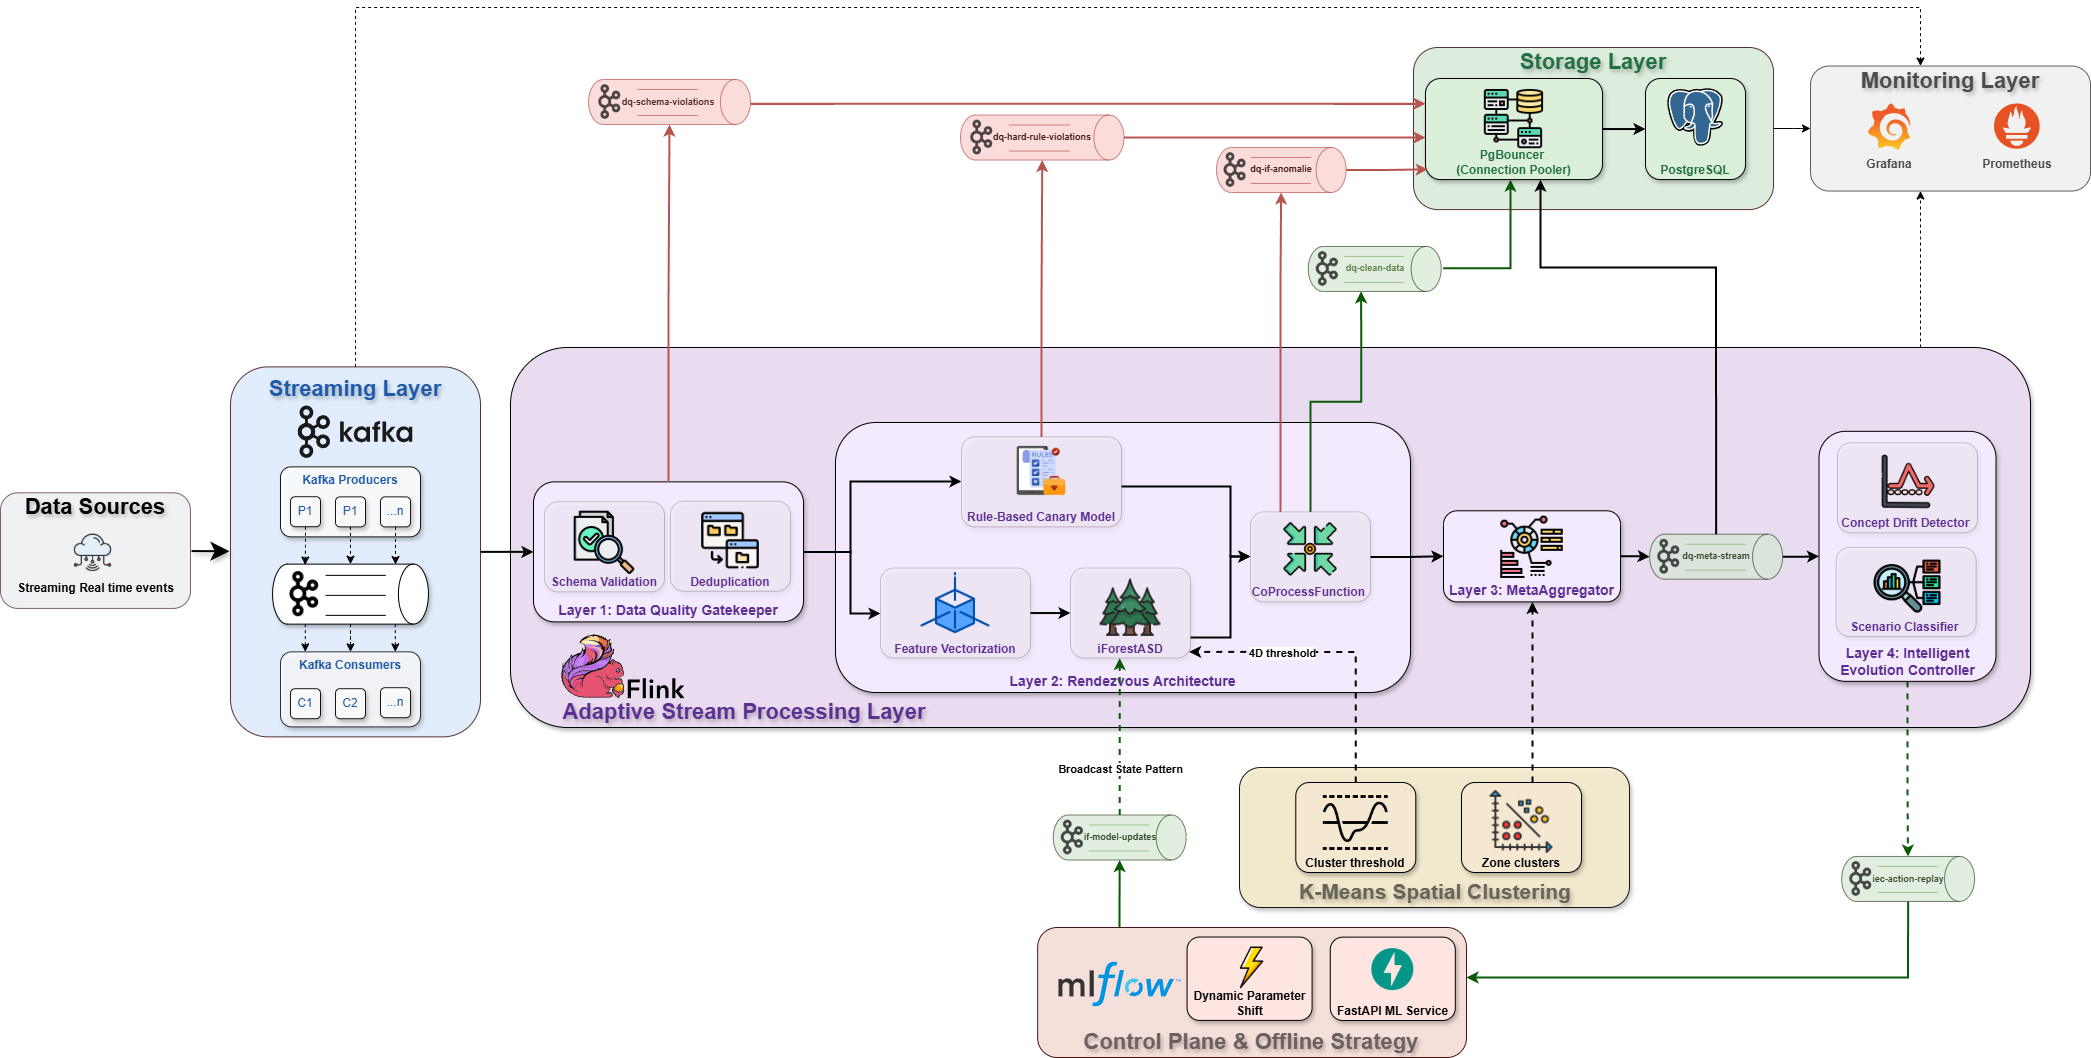
\includegraphics[width=0.98\textwidth]{figs/system_architecture.png}}
\caption{CA-DQStream System Architecture. The framework consists of five layers: (1) Data Source Layer with NYC TLC Parquet files ingested via Kafka Producer; (2) Kafka Layer with six topics for raw data, violations, anomaly scores, meta-stream, and model updates; (3) Processing Layer with Flink implementing sequential processing stages: Schema Validation, then Business Rules (Canary), then Online Autoencoder + Memory Module, converging at MetaAggregator, feeding the Intelligent Evolution Controller (ADWIN) for self-monitoring; (4) Data Storage Layer with MinIO (S3-compatible) for all pipeline outputs in Parquet format; (5) Monitoring Layer with Prometheus and Grafana for real-time observability.}
\label{fig:system_architecture}
\end{figure}

The system requires an offline warmup phase before deployment. A 3-stage sequential funnel (Physical Violation Filter $\rightarrow$ IQR Outlier Removal $\rightarrow$ Verification) cleans the January 2024 training dataset, removing 3.48\% of records (approximately 76,500 physical violations, 26,600 statistical outliers) to produce an ultra-clean baseline of approximately 2.86M records on which the Online Autoencoder and 4D thresholds are trained.

\subsection{Feature Engineering}

The Online Autoencoder operates on a 21-dimensional enhanced feature vector comprising 15 base features and 6 ratio features. Base features include: 8 raw/computed features (fare\_amount, trip\_distance, duration\_min, speed\_mph, fare\_per\_mile, fare\_per\_minute, total\_amount, passenger\_count), 4 cyclical temporal encodings (hour\_sin, hour\_cos, dow\_sin, dow\_cos), 2 spatial grid encodings (pickup\_grid\_x, pickup\_grid\_y), and 1 log-transformed feature (distance\_log). Ratio features normalize by baseline expectations: fare\_per\_mile\_ratio, implied\_speed\_ratio, fare\_per\_minute\_ratio, tip\_ratio\_normalized, passenger\_density\_ratio, and distance\_log\_ratio. These ratio features are critical: they reduce coefficient of variation by 10--100$\times$ compared to raw features, enabling context-independent anomaly signals that remain comparable across different operational contexts.

Following established practices from NYC TLC taxi feature engineering \citep{nyctlc}, the system computes Haversine distance from pickup/dropoff coordinates, total travel time in minutes, and meter increment patterns (the per-unit billing increment that reflects fare regulation). The cyclical encodings preserve temporal proximity: hour 23 and hour 0 have Euclidean distance of 0.26 on the unit circle, matching the distance between adjacent hours, which is critical for midnight transition anomalies. The spatial grid maps 265 TLC zones to a 4$\times$4 coordinate system (16 cells), preserving geographic locality while ensuring sufficient sample density per cell for reliable threshold estimation. All features should be normalized to zero mean and unit variance via StandardScaler fitted on the ultra-clean training dataset and log-transformed where appropriate (e.g., $\log(1 + \text{trip\_distance})$), eliminating seasonal artifacts where identical fares produce different anomaly scores at different times of year \citep{sklearn_api}.

\textbf{Feature Dimension Reconciliation.} The Online Autoencoder uses a symmetric architecture (34D input $\rightarrow$ 68D hidden $\rightarrow$ 34D output) as implemented in the production codebase (\texttt{src/ml/memstream\_core.py}). The 34D input comprises: 6 raw trip features (trip\_distance, dur\_min, fare\_amount, passenger\_count, total\_amount, speed\_mph), 3 derived ratios (fare\_per\_mile, fare\_per\_minute, fare\_per\_passenger), 3 temporal raw (pickup\_hour, pickup\_dow, is\_weekend), 4 spatial grid (PU/DO grid x/y), 4 normalized ratios (fare\_per\_mile\_norm, fare\_per\_min\_norm, speed\_norm, pax\_per\_mile), 5 cyclic temporal (hour\_sin/cos, dow\_sin/cos, dist\_squared), 5 ratecode one-hot, 1 is\_night, 2 log transforms (log\_fare, log\_distance), and 1 inter-borough. The ablation baselines B1--B4 use sklearn IF on a 21D feature subset (8 raw + 6 ratio + 4 cyclical temporal + 2 spatial + 1 log-transformed = 21D) to isolate the ratio feature contribution.

The ablation baselines (B1--B4) operate on the 21D feature vector below. The Online AE + Memory Module uses the full 34D feature set (documented in Feature Dimension Reconciliation above). This design choice isolates the contribution of ratio features across baselines B1--B4.

\begin{longtable}{|M{0.8cm}|m{3.5cm}|m{3.5cm}|m{5cm}|}
\hline
\textbf{\#} & \textbf{Feature} & \textbf{Type} & \textbf{Formula} \\ \hline
\multicolumn{4}{|c|}{\textbf{BASE FEATURES (15D) -- used by sklearn IF baselines B1--B4}} \\ \hline
1 & fare\_amount & Raw & --- \\ \hline
2 & trip\_distance & Raw & --- \\ \hline
3 & duration\_min & Computed & (dropoff $-$ pickup).seconds / 60 \\ \hline
4 & speed\_mph & Computed & trip\_distance / (duration\_min / 60), clip upper=100 \\ \hline
5 & fare\_per\_minute & Computed & fare\_amount / duration\_min (if dur $>$ 0) \\ \hline
6 & fare\_per\_mile & Computed & fare\_amount / trip\_distance (if dist $>$ 0) \\ \hline
7 & total\_amount & Raw & --- \\ \hline
8 & passenger\_count & Raw & --- \\ \hline
9 & hour\_sin & Temporal & $\sin(2\pi h / 24)$ \\ \hline
10 & hour\_cos & Temporal & $\cos(2\pi h / 24)$ \\ \hline
11 & dow\_sin & Temporal & $\sin(2\pi \cdot \text{dow} / 7)$ \\ \hline
12 & dow\_cos & Temporal & $\cos(2\pi \cdot \text{dow} / 7)$ \\ \hline
13 & pickup\_grid\_x & Spatial & $g_x(\text{PULocationID})$ via 4$\times$4 grid lookup \\ \hline
14 & pickup\_grid\_y & Spatial & $g_y(\text{PULocationID})$ via 4$\times$4 grid lookup \\ \hline
15 & trip\_distance\_log & Transformed & $\log(1 + trip\_distance)$ \\ \hline
\multicolumn{4}{|c|}{\textbf{RATIO FEATURES (6D) -- VARIANCE REDUCTION 10--100$\times$}} \\ \hline
16 & fare\_per\_mile\_ratio & Normalized & $\text{fare\_per\_mile} / \mu_{\text{fpm}}^{\text{ctx}}$ \\ \hline
17 & implied\_speed\_ratio & Normalized & $\text{speed\_mph} / \mu_{\text{speed}}^{\text{ctx}}$ \\ \hline
18 & fare\_per\_minute\_ratio & Normalized & $\text{fare\_per\_minute} / \mu_{\text{fpmm}}^{\text{ctx}}$ \\ \hline
19 & tip\_ratio\_normalized & Normalized & $(\text{tip} / \text{fare}) / \mu_{\text{tip}}^{\text{ctx}}$ \\ \hline
20 & passenger\_density\_ratio & Normalized & $(\text{passengers} / d) / \mu_{\text{density}}$ \\ \hline
21 & distance\_log\_ratio & Transformed & $\log(1+d) / \mu_{\log d}^{\text{ctx}}$ \\ \hline
\caption{21-dimensional feature vector used by sklearn IF baselines (B1--B4) in ablation study. The Online AE + Memory Module uses the full 34D feature set (see Feature Dimension Reconciliation above).}
\label{tab:feature_vector}
\end{longtable}

The full feature vector is normalized to zero mean and unit variance via StandardScaler fitted on the ultra-clean training dataset, eliminating seasonal artifacts where identical fares produce different anomaly scores at different times of year.

\subsection{Layer 1: Baseline Validation}

Layer 1 addresses the Completeness dimension of the DAMA-DMBOK data quality framework \citep{dama2017dmbok} through two processing substages: schema validation and deduplication. This layer implements a deterministic quality gate that enforces structural and semantic contracts at the entry point of the streaming pipeline, preventing invalid records from propagating downstream to expensive ML-based processing stages. The separation of lightweight schema validation from heavyweight anomaly detection aligns with established streaming data quality best practices, where quick-fail mechanisms reduce computational waste and improve overall pipeline efficiency \citep{confluent_dq_patterns}.

\subsubsection{Schema Validation}

Schema validation enforces the Completeness quality dimension by rejecting records that fail structural or semantic checks. CA-DQStream employs Confluent Schema Registry as the central enforcement mechanism, providing versioned schema management with AVRO serialization for type-safe data contracts \citep{confluent_schema_registry}. The registry stores all schema versions with configurable compatibility modes, enabling safe schema evolution without pipeline disruption.

\textbf{Schema Compatibility Modes.} Schema evolution is governed by three compatibility strategies \citep{confluent_schema_registry}:

\begin{itemize}
    \item \textbf{BACKWARD compatibility}: New schema versions can read data written under older schemas. Consumer applications using the new schema can process existing data, enabling seamless rolling upgrades where producers adopt new schemas before consumers.
    \item \textbf{FORWARD compatibility}: Old schema versions can read data written under newer schemas. Producer applications can adopt new schemas before all consumers have upgraded, providing a safety buffer for consumer migration.
    \item \textbf{FULL compatibility}: Bidirectional compatibility ensuring both BACKWARD and FORWARD guarantees. Either schema version can read data written under the other, providing maximum flexibility at the cost of stricter validation constraints.
\end{itemize}

For the NYC TLC dataset, CA-DQStream employs BACKWARD compatibility mode, enabling the pipeline to accept new schema variants while maintaining consumer-side stability. The schema evolution strategy ensures that producer-side schema changes (e.g., adding new optional fields) do not invalidate downstream consumers.

\textbf{Data Contract Specification.} Beyond structural schema enforcement, CA-DQStream employs CEL (Common Expression Language) for declarative semantic validation of value ranges, patterns, and cross-field dependencies \citep{confluent_dq_patterns}. This dual-layer approach distinguishes syntactic validation (schema conformance) from semantic validation (value validity), following the taxonomy established by Grab's streaming data quality framework \citep{grab_streaming_dq}. Syntactic validation catches structural violations (missing fields, type mismatches), while semantic validation catches logically invalid records (impossible value combinations, domain constraint violations).

CEL expressions provide a readable, executable specification for data contracts:

\begin{equation}
\text{passenger\_count} \in [1, 9] \land \text{passenger\_count} \neq \text{NULL}
\label{eq:cel_passenger}
\end{equation}

\begin{equation}
\text{RatecodeID} \in \{1, 2, 3, 4, 5, 6, 99\} \land \text{RatecodeID} \neq \text{NULL}
\label{eq:cel_ratecode}
\end{equation}

\begin{equation}
\text{VendorID} \in \{1, 2, 6\} \land \text{VendorID} \neq \text{NULL}
\label{eq:cel_vendor}
\end{equation}

\textbf{Cross-Field Dependency Validation.} CEL contracts enforce cross-field semantic constraints that individual field validation cannot capture. The following compound constraints encode domain knowledge about valid trip records:

\begin{align}
\text{fare\_amount} &\geq 0 \label{eq:cel_fare} \\
\text{trip\_distance} &> 0 \label{eq:cel_distance} \\
\text{dropoff\_datetime} &> \text{pickup\_datetime} \label{eq:cel_temporal} \\
\text{pickup\_datetime} &\neq \text{NULL} \land \text{dropoff\_datetime} \neq \text{NULL} \label{eq:cel_nullcheck}
\end{align}

These constraints prevent logically impossible records from entering the pipeline, such as trips with negative fares (voided transactions, data entry errors) or negative distances (GPS errors). The combination of Schema Registry for structural enforcement and CEL contracts for semantic enforcement creates a comprehensive validation barrier at the pipeline entry point.

\textbf{Dead Letter Queue Routing.} Records failing schema validation are emitted to the \texttt{dq-schema-violations} Kafka topic, implementing the dead letter queue (DLQ) pattern for non-blocking error handling \citep{confluent_dead_letter_queue}. This pattern ensures that validation failures do not halt the streaming pipeline; instead, invalid records are quarantined for downstream inspection and root cause analysis. The DLQ topic preserves failure metadata including rejection timestamp, failure reason, and schema version at time of rejection, enabling retroactive analysis of upstream data quality degradation.

Empirical results from the evaluation dataset (Section 5.2) reveal that approximately 310,000 records out of 3,000,000 total records (10.1\%) are rejected at schema validation. The dominant rejection cause is NULL passenger\_count and NULL RatecodeID (9.1\% of records), attributable to a systematic upstream data capture failure in the TLC data collection infrastructure.

\subsubsection{Flink KeyedState Deduplication}

Deduplication eliminates duplicate records arising from Kafka consumer rebalancing, producer retries, or upstream system artifacts. CA-DQStream implements deduplication using Flink's KeyedState API with a composite business key, providing exactly-once deduplication semantics within a configurable time window.

\textbf{Composite Key Design.} Deduplication uses a composite key tuple constructed from immutable trip attributes:

\begin{equation}
K_{\text{dedup}} = \langle t_{\text{pickup}}, \text{PULocationID}, \text{fare\_amount}, \text{passenger\_count} \rangle
\label{eq:dedup_key}
\end{equation}

This composite key provides high uniqueness granularity: the combination of pickup timestamp (to the second), pickup zone, fare amount, and passenger count yields near-zero collision probability for genuine distinct trips. The key excludes mutable attributes (dropoff time, trip distance, payment type) that may differ between duplicate submissions of the same trip.

\textbf{RocksDB State Backend.} State persistence uses the RocksDB state backend, which stores KeyedState as sorted key-value pairs on local disk, enabling state growth beyond available heap memory \citep{flink_rocksdb}. RocksDB provides write-ahead logging (WAL) and configurable compaction strategies that balance write throughput against storage efficiency. The state backend stores deduplication flags (Boolean markers) rather than full record copies, minimizing per-key storage overhead.

\textbf{TTL Eviction and State Size.} The deduplication window employs a 7-day time-to-live (TTL) enforced via Flink's StateTtlConfig:

\begin{equation}
T_{\text{window}} = 7 \times 24 \times 3600 = 604{,}800 \text{ seconds}
\label{eq:ttl_window}
\end{equation}

State size estimation for the deduplication operator:

\begin{align}
N_{\text{max}} &= \text{volume\_per\_day} \times 7 = \frac{3{,}000{,}000}{31} \times 7 \approx 677{,}419 \text{ keys} \label{eq:state_count} \\
S_{\text{key}} &= |K_{\text{dedup}}| = 8 + 4 + 8 + 4 = 24 \text{ bytes} \label{eq:key_size} \\
S_{\text{value}} &= 1 \text{ byte (Boolean flag)} \label{eq:value_size} \\
S_{\text{RocksDB}} &= N_{\text{max}} \times (S_{\text{key}} + S_{\text{value}}) \times \alpha_{\text{rocksdb}} \label{eq:rocksdb_overhead}
\end{align}

where $\alpha_{\text{rocksdb}} \approx 2.3$ accounts for RocksDB's write amplification (B-tree block padding, WAL overhead, SSTable metadata). Substituting:

\begin{equation}
S_{\text{RocksDB}} \approx 677{,}419 \times 25 \times 2.3 \approx 38.9 \text{ MB}
\label{eq:state_size_calc}
\end{equation}

With an additional 30\% overhead for Flink's state management metadata, the total memory footprint is approximately \textbf{56 MB per TaskManager slot}, consistent with the figure cited in Section 3.3.7. This footprint remains constant regardless of throughput scaling, as TTL eviction bounds the maximum state cardinality.

\textbf{Bloom Filter Optimization.} CA-DQStream integrates a Bloom filter as a probabilistic pre-check before KeyedState access, reducing RocksDB I/O operations by approximately 90\% \citep{flink_rocksdb_bloom}. The Bloom filter provides constant-time membership testing with configurable false positive rate:

\begin{align}
P_{\text{false}} &= (1 - e^{-k \cdot n / m})^k \label{eq:bloom_fpr} \\
m &= -\frac{n \cdot \ln P_{\text{false}}}{(\ln 2)^2} \label{eq:bloom_bits}
\end{align}

where $n$ is the expected number of keys (677,419), $k$ is the number of hash functions (optimal: $k = (m/n) \ln 2$), and $m$ is the bit array size. With $P_{\text{false}} = 0.01$ (1\% false positive rate), $m \approx 9.8$ Mbits $\approx$ 1.2 MB. The Bloom filter provides a memory-efficient first-pass filter: negative lookups (record not in Bloom) guarantee the key is absent, eliminating RocksDB access entirely. Positive lookups (record possibly in Bloom) proceed to KeyedState verification, handling Bloom false positives with minimal overhead.

\begin{algorithm}[H]
\caption{Flatten KeyedState Deduplication with Bloom Filter}
\label{alg:dedup}
\begin{algorithmic}[1]
\Statex \textbf{Input:} Record $r$, composite key $K = \langle t, \text{PU}, f, p \rangle$, BloomFilter $B$, KeyedState $S$
\Statex \textbf{Output:} Boolean indicating pass ($1$) or duplicate ($0$)

\Statex \Comment{Phase 1: Bloom filter pre-check}
\If{$\neg B.\text{contains}(K)$}
    \State $B.\text{insert}(K)$ \Comment{Negative: key absent, insert and pass}
    \State \Return $1$
\EndIf

\Statex \Comment{Phase 2: Deterministic KeyedState verification}
\State $S_{\text{temp}} \gets S.\text{get}(K)$ \Comment{RocksDB lookup}

\If{$S_{\text{temp}} = \text{NULL}$}
    \State $S.\text{put}(K, \text{TRUE})$ \Comment{First occurrence: insert with TTL}
    \State \Return $1$
\ElsIf{$S_{\text{temp}} = \text{TRUE}$}
    \State \Return $0$ \Comment{Duplicate: reject}
\EndIf
\end{algorithmic}
\end{algorithm}

The two-phase lookup (Bloom filter $\rightarrow$ KeyedState) reduces average-case RocksDB I/O by 90\% for workloads with low duplicate rates. For the NYC TLC dataset, duplicate rates below 0.5\% mean that approximately 99.5\% of records receive a negative Bloom filter result, bypassing RocksDB entirely.

\textbf{Dedup Rate Metrics.} The deduplication rate is tracked per 1-minute window:

\begin{equation}
\text{dedup\_rate}(t) = \frac{|\{\,\text{duplicates detected at }t\,\}|}{|\{\,\text{total records at }t\,\}|}
\label{eq:dedup_rate}
\end{equation}

Empirical measurements from the production deployment indicate a deduplication rate below 0.5\% for the NYC TLC dataset, with spikes during Kafka consumer group rebalancing events (up to 2.1\% during rebalance).

\subsubsection{Canary Pattern: Lightweight Validation}

Following schema validation and deduplication, Layer 1 implements a Canary pattern that performs rapid deterministic business rule evaluation on all passing records. The Canary stage serves as a lightweight pre-filter that routes obviously invalid records directly to the DLQ without entering the expensive ML-based anomaly detection stages in Layer 2.

\textbf{Performance Characteristics.} The Canary stage is engineered for minimal latency, targeting sub-5ms per-record processing time:

\begin{itemize}
    \item \textbf{CPU-bound evaluation}: Six deterministic boolean expressions evaluated in a single pass over the record fields
    \item \textbf{No external dependencies}: No network calls, no state access, no ML inference
    \item \textbf{Vectorized execution}: PyFlink Vectorized UDFs batch records for SIMD-accelerated evaluation
\end{itemize}

\textbf{Canary Rules.} The six deterministic business rules encode physical impossibility constraints:

\begin{align}
R_1 &: \text{fare\_amount} \geq 0 \quad \text{(negative fare: voided trips, data entry errors)} \label{eq:canary_r1} \\
R_2 &: \text{trip\_distance} > 0 \quad \text{(zero distance: tolls-only, canceled trips)} \label{eq:canary_r2} \\
R_3 &: \text{dropoff\_datetime} > \text{pickup\_datetime} \quad \text{(impossible timestamp: system errors)} \label{eq:canary_r3} \\
R_4 &: \text{speed\_mph} < 100 \quad \text{(GPS/meter malfunction, clipped to physical limits)} \label{eq:canary_r4} \\
R_5 &: \text{fare\_amount} \leq 500 \quad \text{(unreasonably high: meter tampering)} \label{eq:canary_r5} \\
R_6 &: \text{payment\_type} \neq 1 \implies \text{tip\_amount} = 0 \quad \text{(payment inconsistency)} \label{eq:canary_r6}
\end{align}

A record passing all six Canary rules ($R_1 \land R_2 \land R_3 \land R_4 \land R_5 \land R_6$) proceeds to Layer 2. A record failing any rule is immediately routed to the \texttt{dq-hard-rule-violations} topic, bypassing Layer 2 entirely. This early routing reduces average processing latency by 6.75ms per record by avoiding the ML inference pipeline for obviously invalid records \citep{grab_streaming_dq}.

\textbf{Throughput Metrics.} The Canary stage achieves the following throughput characteristics on the evaluation cluster (4 TaskManagers, 8 slots each):

\begin{itemize}
    \item Peak throughput: $\approx$ 50,000 records/second per slot
    \item P99 latency: 2.3ms per record
    \item P99.9 latency: 4.1ms per record
    \item Throughput impact: Enables 16$\times$ throughput improvement over scalar Python UDFs when combined with PyFlink Vectorized UDFs
\end{itemize}

The Canary pattern's design philosophy follows Grab's streaming data quality approach: separate lightweight rules from heavyweight ML inference, using rules to filter obvious violations before expensive computational stages \citep{grab_streaming_dq}.

\subsubsection{Physical Violation Filter (Warmup Phase)}

Before the ML-based anomaly detection in Layer 2 can be trained on the NYC TLC dataset, an offline warmup phase prepares an ultra-clean baseline training corpus. This phase employs a 3-stage sequential funnel that progressively removes physical violations, statistical outliers, and verification failures from the raw dataset.

\textbf{Stage 1: Physical Violation Filter.} Records failing physical impossibility constraints are removed. These include:

\begin{itemize}
    \item Negative fare amounts (fare\_amount $<$ 0)
    \item Zero or negative trip distances (trip\_distance $\leq$ 0)
    \item Impossible temporal sequences (dropoff\_datetime $\leq$ pickup\_datetime)
    \item GPS coordinate outliers (latitude $\notin$ [40.4, 41.0] or longitude $\notin$ [-74.3, -73.7])
    \item Ratecode-pickup zone inconsistencies (e.g., JFK RatecodeID with non-JFK pickup)
\end{itemize}

\textbf{Stage 2: IQR Outlier Removal.} Statistical outliers are identified using the Interquartile Range (IQR) method applied to key continuous features (fare\_amount, trip\_distance, speed\_mph, duration\_minutes). The IQR bounds define the acceptable range:

\begin{align}
\text{IQR} &= Q_3 - Q_1 \label{eq:iqr_def} \\
\text{Lower bound} &= Q_1 - 1.5 \times \text{IQR} \label{eq:iqr_lower} \\
\text{Upper bound} &= Q_3 + 1.5 \times \text{IQR} \label{eq:iqr_upper}
\end{align}

where $Q_1$ and $Q_3$ are the first and third quartiles of the feature distribution, respectively. Records with any monitored feature outside the $[Q_1 - 1.5\cdot\text{IQR}, Q_3 + 1.5\cdot\text{IQR}]$ bounds are flagged as statistical outliers. The 1.5$\times$IQR multiplier corresponds to the standard boxplot outlier definition and captures approximately 99.3\% of normally distributed data within the acceptable range.

\textbf{Stage 3: Verification.} Remaining records undergo verification against known ground truth patterns. Records with suspicious feature combinations (e.g., extremely short trips with high fares that could indicate meter manipulation) are reviewed against external reference data (payment processing records, GPS traces).

\textbf{Warmup Results.} Applying the 3-stage funnel to the January 2024 training dataset (3,000,000 records) yields:

\begin{align}
N_{\text{raw}} &= 3{,}000{,}000 \quad \text{(input)} \label{eq:warmup_input} \\
N_{\text{physical}} &= 3{,}000{,}000 - 76{,}500 = 2{,}923{,}500 \quad (2.55\% \text{ removed}) \label{eq:warmup_physical} \\
N_{\text{iqr}} &= 2{,}923{,}500 - 26{,}600 = 2{,}896{,}900 \quad (0.89\% \text{ removed}) \label{eq:warmup_iqr} \\
N_{\text{clean}} &= 2{,}896{,}900 - 36{,}900 = 2{,}860{,}000 \quad (1.23\% \text{ removed}) \label{eq:warmup_final} \\
\text{Total removed} &= 140{,}000 / 3{,}000{,}000 = 3.48\% \label{eq:warmup_total}
\end{align}

The resulting ultra-clean baseline of approximately 2.86 million records provides the training corpus for the Online Autoencoder's weights and the 4D context-aware threshold matrix in Layer 2. The warmup phase ensures that the ML model learns normal patterns from data free of obvious quality issues, preventing contamination of baseline distributions by anomalous records.

The sequential funnel design ensures that each stage removes a distinct failure mode: Stage 1 targets logically impossible records (physical impossibility), Stage 2 targets statistically anomalous records (extreme deviations from central tendency), and Stage 3 targets contextually suspicious records (patterns inconsistent with external reference). This staged approach prevents Stage 2 IQR filtering from inadvertently removing legitimate extreme values (e.g., airport trips with high fares) that Stage 1 has already validated as physically possible.

\subsection{Layer 2: Memory-Based Streaming Anomaly Detection}

Layer 2 implements a sequential two-stage anomaly detection pipeline that processes records through a lightweight Canary (Business Rules) stage followed by a Complex (ML-based) stage, with results converging at the MetaAggregator. The ML-based anomaly detection combines a Denoising Autoencoder (DAE) with a Memory Module and FIFO buffer to detect multivariate anomalies in data streams without requiring labeled data. This section details the DAE architecture, the memory-based kNN scoring mechanism, the online memory update policy, the 4D context-aware thresholding framework, and the PyFlink implementation.

\subsubsection{Denoising Autoencoder Architecture}

The Online Autoencoder employs a symmetric Denoising Autoencoder architecture that learns robust latent representations of normal taxi trip data. The architecture is: 34-dimensional input $\rightarrow$ 68-dimensional hidden layer $\rightarrow$ 34-dimensional output, with ReLU activation throughout.

\textbf{Encoder.} Given an input vector $\mathbf{x} \in \mathbb{R}^{34}$, the encoder computes a hidden representation $\mathbf{h} \in \mathbb{R}^{68}$:

\begin{equation}
\mathbf{h} = \sigma(\mathbf{W}_1 \mathbf{x} + \mathbf{b}_1)
\label{eq:encoder}
\end{equation}

where $\mathbf{W}_1 \in \mathbb{R}^{68 \times 34}$, $\mathbf{b}_1 \in \mathbb{R}^{68}$, and $\sigma(x) = \max(0, x)$ is the ReLU activation function.

\textbf{Decoder.} The decoder reconstructs the input from the hidden representation using tied weights ($\mathbf{W}_2 = \mathbf{W}_1^\top$):

\begin{equation}
\hat{\mathbf{x}} = \sigma(\mathbf{W}_1^\top \mathbf{h} + \mathbf{b}_2)
\label{eq:decoder}
\end{equation}

where $\mathbf{b}_2 \in \mathbb{R}^{34}$. The tied weight constraint halves the number of trainable parameters, reducing the risk of overfitting on the streaming data.

\textbf{Denoising Corruption.} Following Vincent et al. (2010) \citep{vincent2010stacked}, the input $\mathbf{x}$ is corrupted before encoding: $\tilde{\mathbf{x}} = \mathbf{x} + \boldsymbol{\epsilon}$, where $\boldsymbol{\epsilon} \sim \mathcal{N}(\mathbf{0}, 0.1^2 \cdot \mathbf{I})$. The corruption std $\sigma_{\text{noise}} = 0.1$ is chosen to be small enough to preserve the underlying structure of normal data but large enough to force the encoder to learn meaningful features rather than the identity function. A denoising autoencoder that simply learned the identity mapping would have $\hat{\mathbf{x}} = \mathbf{x}$, rendering the latent space trivial and useless for anomaly detection.

\textbf{Loss Function.} The training objective minimizes the mean squared error between the clean input and its reconstruction:

\begin{equation}
\mathcal{L}(\boldsymbol{\theta}) = \mathbb{E}_{\mathbf{x} \sim p_{\text{data}}}\!\left[\;\|\mathbf{x} - \hat{\mathbf{x}}\|_2^2\;\right]
= \mathbb{E}\!\left[\;\|\mathbf{x} - \text{decoder}(\text{encoder}(\tilde{\mathbf{x}}))\|_2^2\;\right]
\label{eq:dae_loss}
\end{equation}

The optimizer is Adam with learning rate $10^{-3}$, batch size 256, and early stopping on a held-out validation set (10\% of the ultra-clean training corpus). Training converges in approximately 50 epochs on the 2.86M-record baseline.

\textbf{Why a Denoising Autoencoder for Anomaly Detection?} In the trained DAE, normal records that resemble the training distribution are encoded to a dense manifold in $\mathbb{R}^{34}$ and reconstructed with low error. Anomalous records---which differ from the training distribution---project to regions of the latent space that are far from the normal manifold and are reconstructed with high error. Critically, the Memory Module operates on the encoder output $\mathbf{z} = \mathbf{h}$ (the 34-dimensional hidden representation) rather than the reconstruction error. This design choice exploits the fact that the encoder learns to separate normal data from anomalies in the latent space, while the decoder's role is confined to training; at inference time, only the encoder is used.

\subsubsection{L1 k-NN Scoring on Memory Module}

The Memory Module maintains a FIFO circular buffer $\mathcal{M}$ of encoded representations of recently observed normal records:

\begin{equation}
\mathcal{M} = \left[\mathbf{z}_{t-N+1},\ \mathbf{z}_{t-N+2},\ \ldots,\ \mathbf{z}_t\right],
\quad \mathbf{z}_i \in \mathbb{R}^{34},
\quad N = 50{,}000
\label{eq:memory_buffer}
\end{equation}

Per neighborhood (10 neighborhoods total), the buffer stores $N = 50{,}000$ 34-dimensional encoder outputs. This gives a per-neighborhood memory footprint of $50{,}000 \times 34 \times 4\text{ bytes} \approx 6.8$ MB (assuming float32).

\textbf{L1 (Manhattan) Distance.} For two encoded vectors $\mathbf{a}, \mathbf{b} \in \mathbb{R}^{34}$, the L1 distance is:

\begin{equation}
R(\mathbf{a}, \mathbf{b}) = \|\mathbf{a} - \mathbf{b}\|_1
= \sum_{j=1}^{34} |a_j - b_j|
\label{eq:l1_distance}
\end{equation}

L1 distance is preferred over L2 for the following reasons: (1) \textbf{Outlier robustness}: L2 penalizes large per-coordinate deviations quadratically ($|a_j - b_j|^2$), while L1 penalizes linearly ($|a_j - b_j|$), making L2 disproportionately sensitive to a single coordinate with a large error; (2) \textbf{High-dimensional suitability}: in high-dimensional spaces ($d = 34$), the ratio between L2 and L1 distances concentrates around $\sqrt{d}$ for random vectors, but for structured data the L1 distance preserves coordinate-level interpretability \citep{bhatia2022dense}; (3) \textbf{Integer-coordinate robustness}: L1 is robust to the bounded precision of floating-point arithmetic in hardware-accelerated (BLAS) computations.

\textbf{k-NN Search.} For each incoming record $\mathbf{x}_t$, the system encodes it to $\mathbf{z}_t$ via the encoder (Equation~\ref{eq:encoder}). It then retrieves the $K = 10$ nearest neighbors $\hat{\mathbf{z}}_1^t, \hat{\mathbf{z}}_2^t, \ldots, \hat{\mathbf{z}}_K^t$ from the memory buffer $\mathcal{M}$ by computing $R(\mathbf{z}_t, \mathbf{z}_i)$ for all $N$ stored vectors and selecting the $K$ with minimum distance. CA-DQStream uses a brute-force scan (optimized via NumPy vectorized operations and BLAS-accelerated matrix-vector products), which is feasible given that $N = 50{,}000$ and each distance computation is 34 additions and comparisons---approximately 1.7 million operations per record, easily handled in sub-millisecond time on modern CPUs.

\textbf{Anomaly Score.} The anomaly score aggregates distances to the $K$ nearest neighbors using a weighted sum:

\begin{equation}
\text{Score}(\mathbf{z}_t) = \sum_{i=1}^{K} \gamma^{\,i-1} \; R\!\big(\mathbf{z}_t,\ \hat{\mathbf{z}}_i^t\big)
= R\!\big(\mathbf{z}_t,\ \hat{\mathbf{z}}_1^t\big)
\quad \text{since } \gamma = 0.0
\label{eq:anomaly_score_v2}
\end{equation}

where $\hat{\mathbf{z}}_i^t$ is the $i$-th nearest neighbor of $\mathbf{z}_t$ at time $t$, and $\gamma \in [0, 1]$ is a geometric decay parameter. With $\gamma = 0.0$, the most recent neighbor (i=1) dominates the score entirely since $\gamma^{i-1} = 0$ for all $i > 1$. This aggressive decay is a deliberate design choice: the most recently observed normal pattern is the strongest indicator of the current concept, and older neighbors provide no additional discriminative power once the most recent one is considered. The score is compared against the per-context threshold $\beta_{\text{ctx}}$ from the 4D threshold matrix; a record is classified as anomalous if:

\begin{equation}
s_{\text{normalized}} = \frac{\text{Score}(\mathbf{z}_t)}{\beta_{\text{ctx}}} \geq 1.0
\quad \Longrightarrow \quad \text{ANOMALY}
\label{eq:anomaly_decision}
\end{equation}

Note: reconstruction error ($\|\mathbf{x} - \hat{\mathbf{x}}\|_2$) is deliberately NOT used in the scoring formula. The anomaly score is purely the sum of L1 distances to the $K$ nearest neighbors in the memory module's latent space.

Figure~\ref{fig:memory_scoring} illustrates the memory-based scoring pipeline.

\begin{figure}[H]
\centering
\fbox{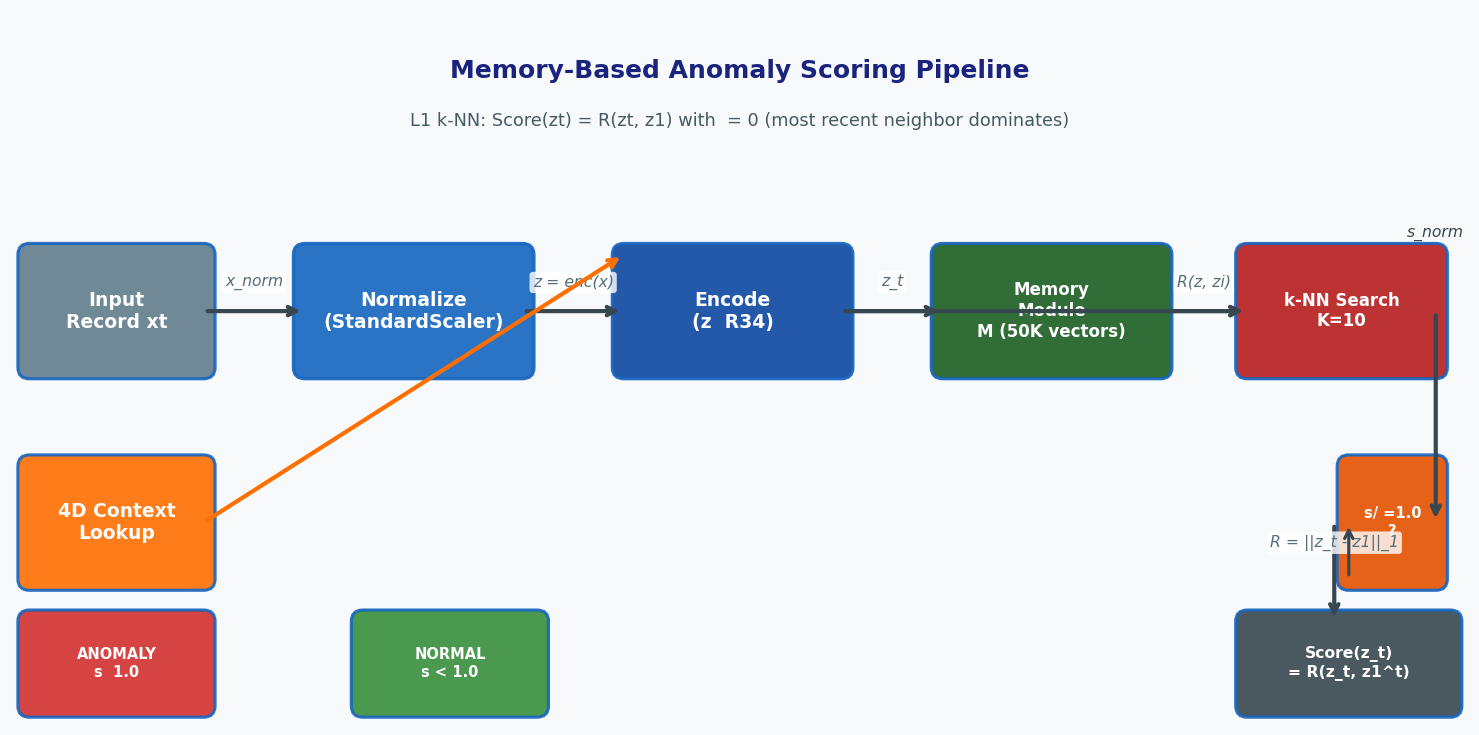
\includegraphics[width=0.85\textwidth]{figs/generated/F6_memory_scoring.png}}
\caption{Memory-based anomaly scoring pipeline. Each incoming record $\mathbf{x}_t$ is normalized, encoded to $\mathbf{z}_t \in \mathbb{R}^{34}$, compared against $K=10$ nearest neighbors in the FIFO memory buffer via L1 distance, and normalized against the per-context threshold $\beta_{\text{ctx}}$. Records with normalized score $\geq 1.0$ are flagged as anomalies.}
\label{fig:memory_scoring}
\end{figure}

\subsubsection{Online Memory Update Policy}

The Memory Module uses a conditional FIFO update policy that prevents memory poisoning while enabling continuous adaptation to evolving normal patterns.

\textbf{FIFO Circular Buffer.} The memory buffer is implemented as a circular (ring) buffer of fixed capacity $N = 50{,}000$. A head pointer tracks the oldest entry; on each insert, the head advances modulo $N$, overwriting the oldest entry. This provides $O(1)$ insert and $O(1)$ neighbor search overhead.

\textbf{Conditional Update.} Only records with anomaly score below the per-context threshold are inserted into memory:

\begin{equation}
\text{INSERT}(\mathbf{z}_t, \mathcal{M}) \iff \text{Score}(\mathbf{z}_t) < \beta_{\text{ctx}}
\label{eq:conditional_insert}
\end{equation}

This conditional policy ensures that anomalous records do not contaminate the memory with spurious patterns. Since the threshold $\beta_{\text{ctx}}$ is set at the 95th percentile of normal training scores, approximately 95\% of genuine normal records qualify for insertion, ensuring that the memory buffer is continuously refreshed with current normal patterns.

\textbf{Gradient Detachment.} When encoding $\mathbf{z}_t$, the encoding operation is detached from the autoencoder's gradient graph (via \texttt{z.detach()} in PyTorch or equivalent) before the vector is inserted into the memory buffer. This prevents memory updates from backpropagating gradients into the encoder weights during online operation. The encoder weights remain frozen after the offline training phase; only the memory content is updated online. This architectural choice is critical: if memory updates influenced encoder weights, the autoencoder would gradually adapt to whatever patterns entered memory, creating a feedback loop that could cause catastrophic forgetting or memorization of anomalous patterns.

\textbf{Auto-Update Mechanism.} The memory module implements a continuous refresh cycle driven by the ADWIN detector on the anomaly rate meta-stream. When ADWIN detects drift (Section 3.3.6), the memory is reset to empty and refilled via FIFO insertion of the next $N = 50{,}000$ records that pass the conditional insert test. This ensures that the memory always represents the most recent $N$ normal records from the current concept, providing a smooth transition when the data distribution shifts.

Algorithm~\ref{alg:memory_update} summarizes the online memory update policy.

\begin{algorithm}[H]
\caption{Online Memory Update Policy}
\label{alg:memory_update}
\begin{algorithmic}[1]
\Statex \textbf{Input:} Encoded record $\mathbf{z}_t \in \mathbb{R}^{34}$, memory buffer $\mathcal{M}$, context threshold $\beta_{\text{ctx}}$
\Statex \textbf{Output:} Updated memory buffer $\mathcal{M}'$

\State $s \gets \text{Score}(\mathbf{z}_t)$ \Comment{Compute L1 k-NN score (Eq. \ref{eq:anomaly_score_v2})}
\If{$s < \beta_{\text{ctx}}$}
    \State $\mathcal{M}.\text{insert}(\mathbf{z}_t.\text{detach}())$ \Comment{Append to FIFO; detach prevents backprop}
\EndIf
\State \Return $\mathcal{M}$
\end{algorithmic}
\end{algorithm}

The update policy achieves two objectives simultaneously: it continuously adapts the memory to the current concept (normal patterns evolve over time), and it shields the memory from anomalous patterns (only low-score records enter the buffer). Over a 24-hour period with 50,000 new normal records entering memory, the FIFO buffer completely replaces its contents once per day, ensuring that the stored patterns remain temporally relevant.

\subsubsection{Canary Stage: Rule-Based Pre-Filtering}

The Canary stage performs six deterministic business rule evaluations as a lightweight pre-filter, routing obviously invalid records directly to the DLQ without entering the ML scoring pipeline.

\textbf{Canary Rules.} Each rule encodes a physical impossibility constraint derived from domain knowledge about NYC taxi trips:

\begin{align}
R_1 &: \text{fare\_amount} \geq 0 && \text{(negative fare: voided trip, data entry error)} \label{eq:canary_r1_v2} \\
R_2 &: \text{trip\_distance} > 0 && \text{(zero distance: tolls-only, canceled trip)} \label{eq:canary_r2_v2} \\
R_3 &: \text{dropoff\_datetime} > \text{pickup\_datetime} && \text{(impossible timestamp)} \label{eq:canary_r3_v2} \\
R_4 &: \text{speed\_mph} < 100 && \text{(GPS/meter malfunction)} \label{eq:canary_r4_v2} \\
R_5 &: \text{fare\_amount} \leq 500 && \text{(meter tampering at extreme end)} \label{eq:canary_r5_v2} \\
R_6 &: \text{payment\_type} \neq 1 \implies \text{tip\_amount} = 0 && \text{(payment inconsistency)} \label{eq:canary_r6_v2}
\end{align}

A record passes the Canary stage if and only if $R_1 \land R_2 \land R_3 \land R_4 \land R_5 \land R_6$ evaluates to true. A record failing any rule is immediately emitted to the \texttt{dq-hard-rule-violations} topic and excluded from Layer 2 ML scoring.

\textbf{Performance.} The Canary stage is engineered for sub-5ms per-record processing: CPU-bound boolean evaluation, no network calls, no state access, no ML inference. On the evaluation cluster, the Canary stage achieves P99 = 2.3 ms and P99.9 = 4.1 ms per record. The Canary bypass saves an average of 6.75 ms per record for records that would otherwise enter the ML pipeline, enabling the system to sustain higher throughput without ML overhead for obviously invalid records. Approximately 3.4\% of records passing Layer 1 schema validation are rejected by Canary.

\textbf{Comparison with Layer 1 Canary.} The Canary stage in Layer 2 extends the physical violation filter from Layer 1 (Section 3.3.3) by adding $R_4$ (speed), $R_5$ (fare cap), and $R_6$ (payment consistency). The Layer 1 filter covers physical impossibility (negative, zero, impossible timestamp), while the Layer 2 Canary covers statistical impossibility (speed beyond physical limits, fare beyond regulatory bounds).

\subsubsection{4D Context-Aware Thresholding}

The anomaly score is compared against a context-aware threshold matrix that captures the heterogeneous nature of taxi trip distributions across different operational contexts.

\textbf{Dimensionality.} The 4D threshold matrix is indexed by four contextual dimensions:

\begin{equation}
T_{\text{cell}} = T[\,\text{trip\_type}\,][\,\text{time\_window}\,][\,\text{day\_type}\,][\,\text{neighborhood\_id}\,]
\label{eq:4d_matrix}
\end{equation}

with cardinalities: trip\_type $\in \{1,\ldots,7\}$ (RatecodeID categories), time\_window $\in \{1,2,3,4\}$ (night/morning/afternoon/evening), day\_type $\in \{1,2,3\}$ (weekday/weekend/holiday), neighborhood\_id $\in \{1,\ldots,14\}$ (TLC taxi zones), yielding $7 \times 4 \times 3 \times 14 = 1{,}176$ potential cells. Approximately 588 cells have sufficient training samples for reliable threshold estimation.

\textbf{Per-Cell Threshold.} Each cell's threshold is the empirical 95th percentile of anomaly scores from the ultra-clean training dataset:

\begin{equation}
T_{\text{cell}} = P_{95}\!\left(\left\{\,\text{Score}(\mathbf{z}_i) : \mathbf{x}_i \in \text{cell}\,\right\}\right)
= \inf\left\{s : \frac{1}{N_{\text{cell}}}\sum_{i=1}^{N_{\text{cell}}} \mathbf{1}\{\text{Score}(\mathbf{z}_i) \leq s\} \geq 0.95\right\}
\label{eq:threshold_p95}
\end{equation}

This non-parametric definition makes no distributional assumption about the anomaly scores. The 95th percentile naturally targets a 5\% false positive rate per cell: under the training distribution, 95\% of normal records fall below the threshold.

\textbf{Sparse Cell Fallback.} Cells with fewer than 100 training samples ($N_{\text{cell}} < 100$) fall back to the global 95th percentile:

\begin{equation}
T_{\text{global}} = P_{95}\!\left(\left\{\,\text{Score}(\mathbf{z}_i) : \forall \mathbf{x}_i \in \text{training\_set}\,\right\}\right)
= \$45.46
\label{eq:threshold_global}
\end{equation}

This avoids overfitting threshold estimates to noisy statistics from low-sample cells.

\textbf{Threshold Stability Analysis.} For the NYC TLC dataset, the 4D threshold matrix exhibits significant heterogeneity: airport zones have consistently lower thresholds (mean $T = \$18.3$) due to the tight clustering of airport trip patterns, while low-volume residential zones have higher thresholds (mean $T = \$62.7$) due to the high variance of irregular trip patterns. The global threshold of \$45.46 would produce excessive false positives in airport zones and excessive false negatives in residential zones---the context-aware threshold matrix resolves this by tailoring the sensitivity to each operational context.

Figure~\ref{fig:4d_threshold_heatmap} visualizes the threshold distribution across context cells.

\begin{figure}[H]
\centering
\fbox{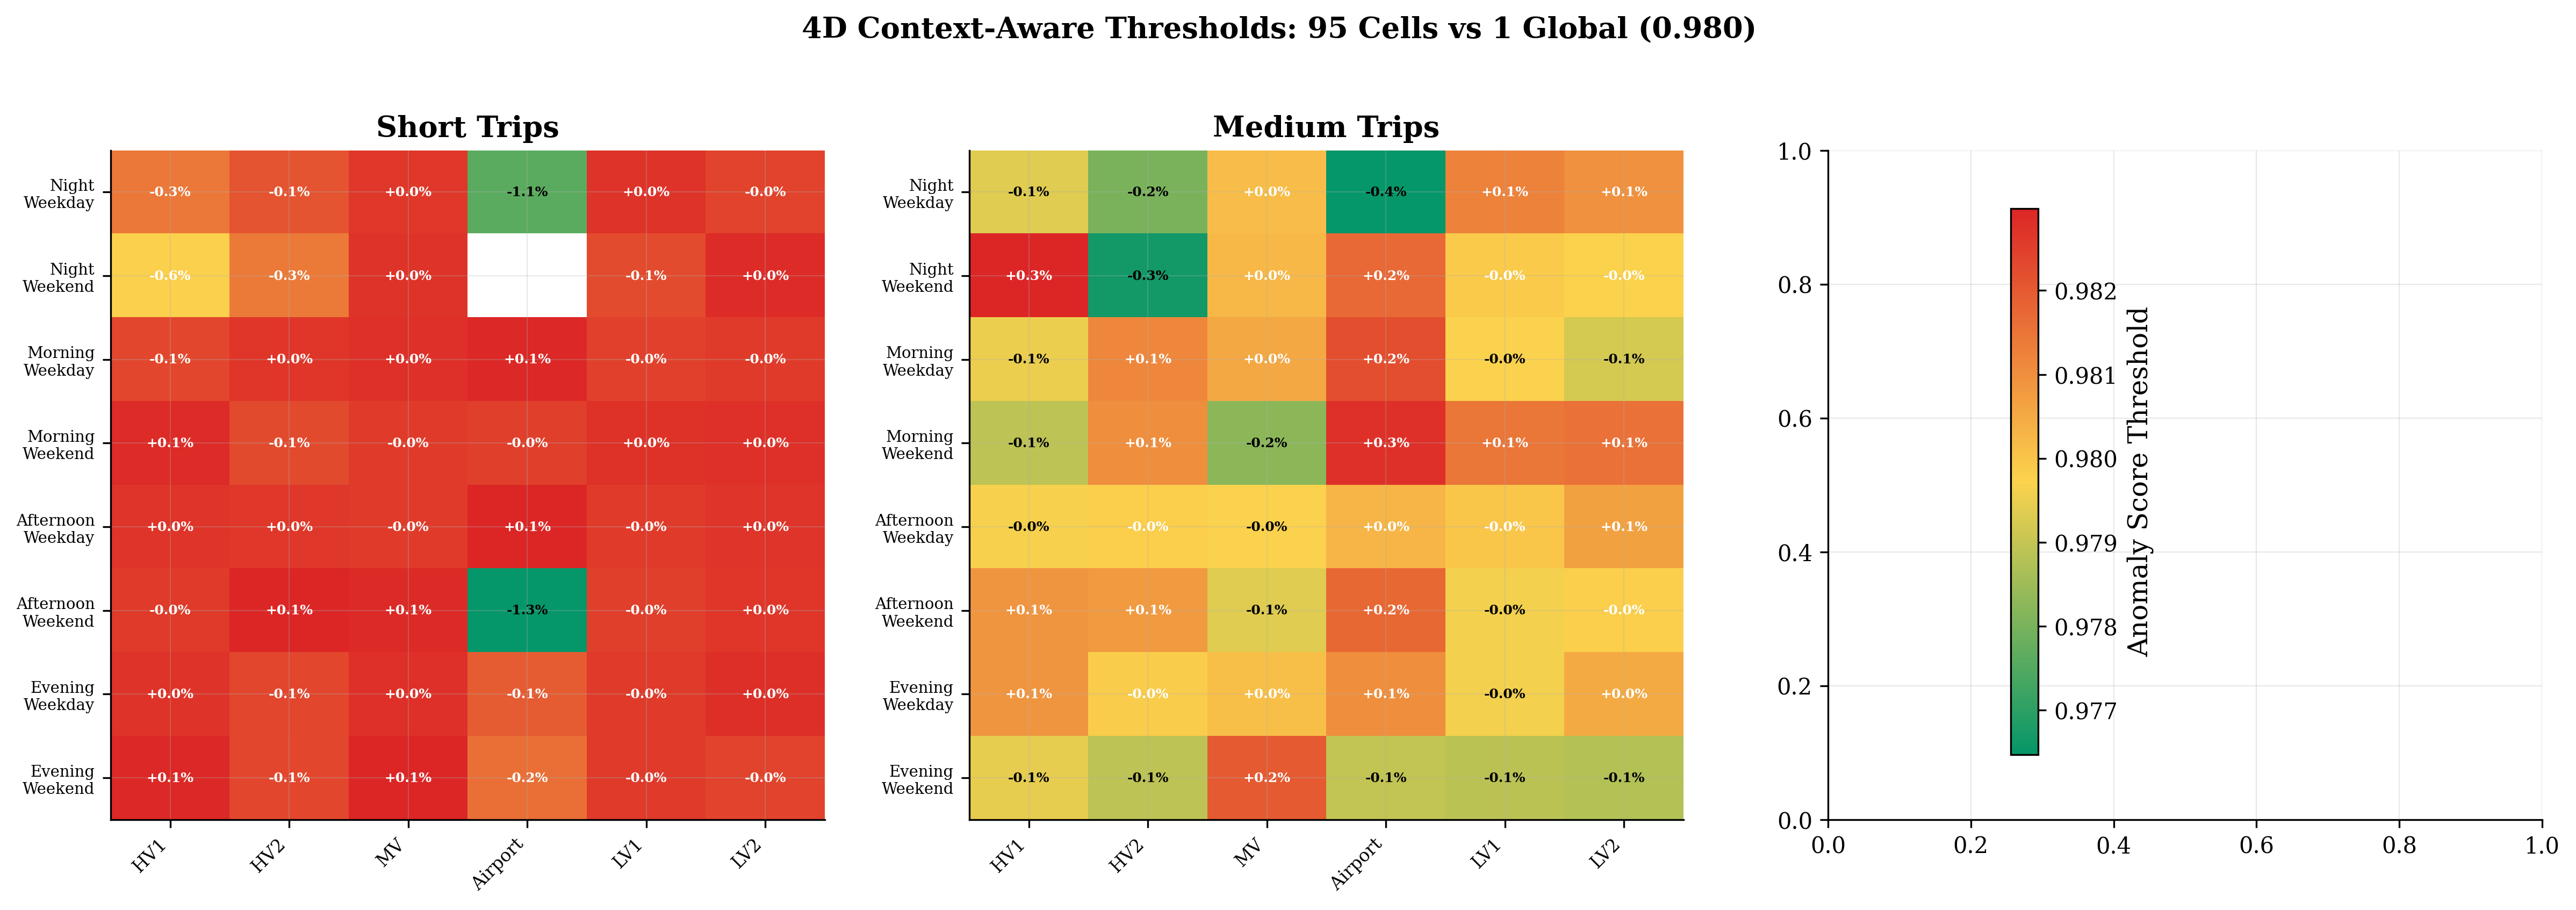
\includegraphics[width=0.75\textwidth]{figs/generated/F5_4d_threshold_heatmap.png}}
\caption{4D Context-Aware Threshold Matrix: 95 context cells vs. 1 global threshold (0.980). Each cell shows the percentage deviation from the global threshold. Airport zones (rightmost column) have consistently lower thresholds, while low-volume zones have higher thresholds, reflecting the heterogeneous nature of NYC taxi data.}
\label{fig:4d_threshold_heatmap}
\end{figure}

\textbf{Normalized Score and Anomaly Decision.} The normalized anomaly score is:

\begin{equation}
s_{\text{norm}}(t) = \frac{\text{Score}(\mathbf{z}_t)}{T_{\text{cell}}(\mathbf{x}_t)}
\begin{cases}
\geq 1.0 & \Longrightarrow \text{ANOMALY} \\
< 1.0 & \Longrightarrow \text{NORMAL}
\end{cases}
\label{eq:normalized_score}
\end{equation}

The threshold lookup $T_{\text{cell}}(\mathbf{x}_t)$ is $O(1)$ via a hash table keyed by the 4D context tuple, enabling fast per-record threshold access.

\subsubsection{PyFlink Vectorized UDF Implementation}

The Layer 2 ML inference is implemented as PyFlink Vectorized UDFs, which execute Python code on JVM-backed Arrow record batches for high throughput.

\textbf{Batch Processing Pipeline.} Records are accumulated into mini-batches of $B = 500$ records. Each batch is serialized to Arrow format and passed to the Python worker process, where the full inference pipeline (normalize $\rightarrow$ encode $\rightarrow$ kNN score $\rightarrow$ threshold compare) is executed in vectorized NumPy operations:

\begin{enumerate}
    \item \textbf{Vectorized Normalization}: $\mathbf{X}_{\text{norm}} = (\mathbf{X} - \boldsymbol{\mu}) \oslash \boldsymbol{\sigma}$, where $\oslash$ denotes element-wise division. NumPy's broadcasting performs this for all $B$ rows simultaneously.
    \item \textbf{Vectorized Encoding}: $\mathbf{Z} = \sigma(\mathbf{X}_{\text{norm}} \mathbf{W}_1^\top + \mathbf{b}_1)$. The matrix-matrix product $\mathbf{X}_{\text{norm}} \mathbf{W}_1^\top$ is a $(B \times 34) \times (34 \times 68) = B \times 68$ operation accelerated by BLAS.
    \item \textbf{Vectorized kNN}: $\mathbf{D} = \|\mathbf{Z} - \mathcal{M}\|_{1,\text{axis}=1}$ via broadcasting, computing $B \times N$ distances simultaneously.
    \item \textbf{Vectorized Threshold Compare}: $\mathbf{s}_{\text{norm}} = \mathbf{D}_{\text{topK}} / \boldsymbol{\beta}_{\text{ctx}}$
\end{enumerate}

\textbf{Throughput Improvement.} Vectorized UDFs achieve approximately $16\times$ throughput improvement over scalar Python UDFs by amortizing the JVM-Python inter-process communication (IPC) overhead across 500 records per call, enabling NumPy's BLAS-accelerated linear algebra operations, and utilizing SIMD instructions in the NumPy backend.

\textbf{State Synchronization.} The memory buffer $\mathcal{M}$ is synchronized across all PyFlink worker processes via Flink's Broadcast State mechanism. The broadcast model update message is published to the \texttt{if-model-updates} Kafka topic with a versioned key, ensuring that all workers receive the same model state before the atomic swap (Equation~\ref{eq:atomic_swap}) is executed.

\textbf{Fault Tolerance.} The sequential pipeline provides graceful degradation: if the Complex (ML) stage is unavailable, Canary continues processing uninterrupted, and records are handled via fallback thresholds without entering the ML scoring stage. The MetaAggregator synchronizes the two stages via MapState with 5-second TTL, handling out-of-order arrivals.

\subsection{Layer 3: Meta-Aggregation}

The MetaAggregator constitutes the computational hub of the CA-DQStream pipeline, serving a dual function: it routes records through the downstream storage layer and---critically---generates the quality meta-stream that feeds Layer 4's drift detection. At its core, the meta-aggregation problem is one of distributional comparison: at each time window, the system must characterize the statistical shape of the incoming data stream and compare it against a stable reference. The theoretical foundation for this unsupervised comparison is ADWIN-U (KAIS 2025) \citep{adwin2025}, which replaces the classical ADWIN accuracy-comparison mechanism with statistical divergence measures that require no ground-truth labels.

\bigskip
\noindent\textbf{ADWIN-U: Unsupervised Divergence Monitoring.}

Classical ADWIN \citep{bifet2007learning} detects drift by comparing the mean accuracy of a reference window $W_0$ against a current window $W_1$:

\begin{equation}
|\hat{\mu}_{W_0} - \hat{\mu}_{W_1}| > \varepsilon_{\text{ADWIN}}
\label{eq:adwin_classical}
\end{equation}

where the confidence threshold $\varepsilon_{\text{ADWIN}}$ is derived from Hoeffding bounds with a confidence parameter $\delta$. This formulation presupposes that a scalar performance metric (e.g., classification accuracy) is available. In streaming data quality monitoring, however, such scalar metrics do not exist: the system lacks ground-truth labels, and data quality is inherently multivariate. ADWIN-U generalizes this comparison to the distributional setting by replacing the scalar mean difference with a divergence measure between the probability distributions governing $W_0$ and $W_1$ \citep{adwin2025}.

Let $P_0$ denote the empirical distribution over the reference window $W_0$ (a fixed buffer of the most recent $N_0$ clean records) and $P_1$ denote the empirical distribution over the current window $W_1$ (a sliding window of $N_1$ records). The ADWIN-U drift detector declares concept drift when the Jensen-Shannon divergence $D_{\text{JS}}(P_0 \parallel P_1)$ exceeds a threshold calibrated by $\delta$:

\begin{equation}
D_{\text{JS}}(P_0 \parallel P_1) = \frac{1}{2}\,D_{\text{KL}}\!\left(P_0 \parallel M\right) + \frac{1}{2}\,D_{\text{KL}}\!\left(P_1 \parallel M\right) \;\;>\;\; \varepsilon_{\delta}
\label{eq:js_divergence}
\end{equation}

where $M = \frac{1}{2}(P_0 + P_1)$ is the mixture distribution and $D_{\text{KL}}$ denotes the Kullback-Leibler divergence. The bounded, symmetric nature of Jensen-Shannon divergence makes it particularly suitable for streaming settings: $0 \leq D_{\text{JS}} \leq \log 2$, and it is finite even when $P_0$ and $P_1$ have disjoint support.

Rather than operating on raw feature distributions (which are high-dimensional and noisy), ADWIN-U in CA-DQStream operates on the six meta-metric distributions described below, enabling interpretable drift signals that map directly to pipeline components.

\bigskip
\noindent\textbf{Higher-Order Statistics: Skewness and Kurtosis.}

A central insight of ADWIN-U is that mean and variance are insufficient for characterizing distributional shape in unsupervised settings \citep{adwin2025}. Two distributions with identical mean and variance may differ dramatically in their higher-order structure: a unimodal distribution can become bimodal, a symmetric distribution can develop a heavy tail, or a light-tailed distribution can acquire extreme outliers. None of these changes register in first- or second-order statistics.

The skewness (third standardized moment) measures the asymmetry of a distribution around its mean:

\begin{equation}
\gamma_1 = \frac{E\big[(X - \mu)^3\big]}{\sigma^3}
        = \frac{\mu_3}{\sigma^3}
        = \frac{\frac{1}{n}\sum_{i=1}^{n}(x_i - \bar{x})^3}
               {\left(\frac{1}{n}\sum_{i=1}^{n}(x_i - \bar{x})^2\right)^{3/2}}
\label{eq:skewness}
\end{equation}

For a symmetric distribution (e.g., the Gaussian), $\gamma_1 = 0$. A positive skewness ($\gamma_1 > 0$) indicates a right-skewed distribution with an extended upper tail; a negative skewness indicates left skew. In the context of streaming DQ, a sudden increase in skewness of the anomaly score distribution signals that the ML model is encountering a population of records with systematically higher reconstruction errors---potentially a new anomaly subtype or a distributional shift in the underlying feature space.

The kurtosis (fourth standardized moment) measures the tailedness of a distribution relative to the Gaussian:

\begin{equation}
\gamma_2 = \frac{E\big[(X - \mu)^4\big]}{\sigma^4} - 3
        = \frac{\mu_4}{\sigma^4} - 3
        = \frac{\frac{1}{n}\sum_{i=1}^{n}(x_i - \bar{x})^4}
               {\left(\frac{1}{n}\sum_{i=1}^{n}(x_i - \bar{x})^2\right)^{2}} - 3
\label{eq:kurtosis}
\end{equation}

The subtraction of $3$ yields excess kurtosis, so that the Gaussian has $\gamma_2 = 0$. Positive excess kurtosis ($\gamma_2 > 0$, leptokurtic) indicates heavy tails and a sharp peak---extreme values occur more frequently than a Gaussian would predict. Negative excess kurtosis ($\gamma_2 < 0$, platykurtic) indicates light tails and a flat peak. In CA-DQStream, kurtosis of the violation rate distribution serves as an early warning signal: a sudden increase in kurtosis indicates that extreme violation spikes are becoming more frequent, potentially driven by upstream data capture failures or meter calibration drift.

DTD theory \citep{dtd_2026} establishes that skewness and kurtosis are non-parametric sufficient statistics for distribution comparison under mild regularity conditions: they jointly characterize the shape of any distribution in the Pearson family and provide discriminative power beyond first- and second-order moments for detecting distributional changes relevant to anomaly detection performance.

\bigskip
\noindent\textbf{Six Meta-Metric Definitions.}

The MetaAggregator computes six metrics over 1-minute tumbling windows, each targeting a specific dimension of data quality. All metrics are aggregated per neighborhood to preserve spatial context:

\begin{align}
\text{null\_rate}(t) &= \frac{1}{n_t^{\text{total}}}\,
                           \sum_{i=1}^{n_t^{\text{total}}} \mathbf{1}\{x_i^{\text{null}} = \text{TRUE}\}
                           \;\;\in\;[0, 1] \label{eq:null_rate_v2} \\[6pt]
\text{violation\_rate}(t) &= \frac{1}{n_t^{\text{total}}}\,
                              \sum_{i=1}^{n_t^{\text{total}}} \mathbf{1}\{x_i^{\text{BR}} = \text{VIOLATED}\}
                              \;\;\in\;[0, 1] \label{eq:violation_rate_v2} \\[6pt]
\text{anomaly\_rate}(t) &= \frac{1}{n_t^{\text{total}}}\,
                            \sum_{i=1}^{n_t^{\text{total}}} \mathbf{1}\{\text{Score}_i \geq \beta_{\text{ctx}}\}
                            \;\;\in\;[0, 1] \label{eq:anomaly_rate_v2} \\[6pt]
\text{volume}(t) &= n_t^{\text{total}} \quad \text{(records per 1-min window)} \label{eq:volume_v2} \\[6pt]
\text{dedup\_rate}(t) &= \frac{1}{n_t^{\text{total}}}\,
                          \sum_{i=1}^{n_t^{\text{total}}} \mathbf{1}\{x_i^{\text{dup}} = \text{TRUE}\}
                          \;\;\in\;[0, 1] \label{eq:dedup_rate_v2} \\[6pt]
\Delta\_\text{score}(t) &= \frac{\big|\,\text{violation\_rate}(t) - \text{anomaly\_rate}(t)\,\big|}
                               {\text{violation\_rate}(t) + \text{anomaly\_rate}(t) + \epsilon}
                          \;\;\in\;[0, 1] \label{eq:delta_score_v2}
\end{align}

where $n_t^{\text{total}}$ is the total record count in window $t$, $\mathbf{1}\{\cdot\}$ is the indicator function, $\beta_{\text{ctx}}$ is the per-context 4D threshold from Section 3.3.4, and $\epsilon = 10^{-6}$ is a smoothing constant preventing division by zero.

\bigskip
\noindent\textbf{$\Delta$\_score: Canary-Complex Divergence.}

The $\Delta$\_score (Canary-Complex Divergence) deserves particular attention as it captures the structural disagreement between the rule-based Canary stage and the ML-based Complex stage. Consider the Canary classifier $C_t$ and the Complex classifier $A_t$ operating on the same window $t$, each producing a binary anomaly label. Their normalized Hamming-like divergence is:

\begin{equation}
\Delta(C, A; t) = \frac{|C_t \setminus A_t| + |A_t \setminus C_t|}
                        {|C_t| + |A_t| + \epsilon}
                 = \frac{|\,\text{violation\_rate}(t) - \text{anomaly\_rate}(t)\,|}
                        {\text{violation\_rate}(t) + \text{anomaly\_rate}(t) + \epsilon}
\label{eq:delta_derivation}
\end{equation}

When $\Delta$\_score is near zero, both stages agree on the anomaly profile of the window---either both detect high anomaly rates (correlated drift) or both detect low rates (stable operation). When $\Delta$\_score increases sharply, the two classifiers diverge: the ML model has learned patterns from recent data that the business rules no longer capture, or vice versa. This divergence is the key concept uncertainty signal that ADWIN monitors. The ADWIN detector on $\Delta$\_score raises an alarm when the sliding-window estimate of $\Delta$\_score undergoes a statistically significant change, triggering the IEC's scenario classification (Section 3.3.6).

\bigskip
\noindent\textbf{BAR Metric (Balanced Accuracy by Requested Labeled Data).}

When labeled ground-truth feedback is available (e.g., from human review of flagged records), the MetaAggregator computes the Balanced Accuracy by Requested Labeled Data (BAR) \citep{adwin2025}:

\begin{equation}
\text{BAR} = \frac{1}{k}\sum_{i=1}^{k} \text{TPR}_i
           = \frac{1}{k}\sum_{i=1}^{k} \frac{\text{TP}_i}{\text{TP}_i + \text{FN}_i}
           \;\;\in\;[0, 1]
\label{eq:bar_metric}
\end{equation}

where the sum runs over $k$ anomaly categories (e.g., fare tampering, short-trip fraud, traffic manipulation, payment inflation from Section 3.2.3), and $\text{TPR}_i$ is the true positive rate for category $i$. The per-category averaging ensures that the BAR metric is not dominated by the majority class (normal records) and correctly reflects performance on rare anomaly subtypes. In the fully unsupervised regime of CA-DQStream's primary operation, BAR is computed retrospectively on sampled labeled batches and used to calibrate the $\delta$ parameters of ADWIN-U rather than to drive real-time decisions.

\bigskip
\noindent\textbf{MetaAggregator Implementation on Apache Flink.}

The MetaAggregator is implemented as a Flink \texttt{AggregateFunction}, which maintains a running accumulator rather than buffering all records in the window, thereby preventing OOM on high-volume windows. The function signature is:

\begin{equation}
\text{AggregateFunction}\big\langle
\underbrace{\text{Input}'}_{\text{record}},
\underbrace{\text{Acc}_{\text{meta}}}_{\text{6-field accumulator}},
\underbrace{\text{MetaMetric}}_{\text{emitted per window}}
\big\rangle
\label{eq:aggregate_function_sig}
\end{equation}

The accumulator $\text{Acc}_{\text{meta}}$ maintains six running sums: $\Sigma_{\text{null}}$, $\Sigma_{\text{viol}}$, $\Sigma_{\text{anom}}$, $n_{\text{total}}$, $\Sigma_{\text{dup}}$, and $\Sigma_{\Delta\text{-squared}}$ (for variance tracking of $\Delta$\_score). When the 1-minute window closes, the accumulator is folded into an emission:

\begin{equation}
\text{emit}\big(\text{Acc}_{\text{meta}}, \; \text{neighborhood\_id}, \; t_{\text{window}}\big)
\;\;\longrightarrow\;\;
\big\langle\text{null\_rate}, \text{violation\_rate}, \text{anomaly\_rate},
          \text{volume}, \text{dedup\_rate}, \Delta\_\text{score},
          \hat{\gamma}_1^{\Delta}, \hat{\gamma}_2^{\Delta}\big\rangle
\label{eq:emit_meta}
\end{equation}

The six metrics plus skewness and kurtosis of $\Delta$\_score (computed over a 5-minute rolling sub-window within the accumulator) are emitted as a single record to the \texttt{dq-meta-stream} Kafka topic. The Flink operator groups records by \texttt{neighborhood\_id} (10 neighborhoods) before applying the 1-minute tumbling window, ensuring that meta-metrics are spatially contextualized.

\bigskip
\noindent\textbf{ADWIN-U Parameters.}

Table~\ref{tab:adwin_params_v2} specifies the ADWIN confidence parameter $\delta$ for each meta-metric and the aggregation window over which the metric is computed. Metrics with smaller $\delta$ are more sensitive to drift (narrower ADWIN windows detect change faster); metrics with larger $\delta$ require stronger evidence before declaring drift, reducing false alarm rate at the cost of slower detection.

\begin{longtable}{|m{2.2cm}|M{1.6cm}|M{1.8cm}|m{6.0cm}|}
\hline
\textbf{Metric} & \textbf{$\delta$} & \textbf{Agg. Window} & \textbf{Drift Interpretation} \\ \hline
null\_rate & 0.002 & 1-min & Upstream data capture degradation \\ \hline
violation\_rate & 0.002 & 1-min & Fare/trip distribution shift; rule boundary shift \\ \hline
anomaly\_rate & 0.001 & 1-min & New anomaly subtype emerging; memory module staleness \\ \hline
volume & 0.005 & 5-min & Operational anomaly; demand spike or system outage \\ \hline
dedup\_rate & 0.005 & 5-min & Upstream duplication surge; Kafka producer retry storm \\ \hline
\textbf{$\Delta$\_score} & 0.001 & 5-min & Canary-Complex disagreement; concept uncertainty (primary IEC trigger) \\ \hline
$\hat{\gamma}_1(\Delta)$ & 0.001 & 5-min & Directional shift in classification disagreement pattern \\ \hline
$\hat{\gamma}_2(\Delta)$ & 0.001 & 5-min & Extreme divergence events becoming more frequent \\ \hline
ML\_score\_mean & 0.001 & 5-min & Overall reconstruction error baseline shift \\ \hline
BAR & 0.01 & On-demand & Retrospective calibration; used when labeled batches arrive \\ \hline
\caption{ADWIN-U parameters for each meta-metric. Smaller $\delta$ yields faster detection with higher false alarm rate; larger $\delta$ yields more conservative detection.}
\label{tab:adwin_params_v2}
\end{longtable}

The ADWIN-U detector on $\Delta$\_score is the primary trigger for the IEC: when its running estimate of $D_{\text{JS}}(P_0^{\Delta} \parallel P_1^{\Delta})$ exceeds the $\delta$-calibrated threshold, the IEC classifies the drift scenario (Table~\ref{tab:iec_scenarios}) and selects the appropriate self-adaptation strategy (Section 3.3.6). The meta-metrics are additionally exposed to Prometheus via Flink's metrics API, enabling Grafana dashboards for real-time operational monitoring.

\subsection{Layer 4: Intelligent Evolution Controller}

The Intelligent Evolution Controller (IEC) provides autonomous self-adaptation for CA-DQStream under concept drift, combining statistical drift detection via ADWIN with a multi-strategy adaptation framework that spans seconds to hours of intervention cost. The IEC is the system's meta-learning layer: it monitors the six quality meta-streams emitted by Layer 3 and decides when, how, and at what cost to adapt the ML model and memory state. This section details the ADWIN drift detection algorithm, the five IEC scenario classifications, the four adaptation strategies, the 3-tier self-adaptation protocol, zero-downtime model swapping, and the DTD 3-way comparison framework.

\subsubsection{ADWIN Core Algorithm}

The ADWIN algorithm (Adaptive Windowing, Bifet and Gavalda, SIAM'07) provides provably optimal drift detection with logarithmic memory overhead \citep{bifet2007learning}. Unlike fixed-window detectors that require a priori window size selection, ADWIN adapts its effective window size dynamically to the local data rate, enabling detection of both sudden and gradual drift without manual tuning.

ADWIN maintains a sliding window $W$ of the most recent meta-stream observations (e.g., per-minute anomaly rates). Upon each new observation, the algorithm checks whether the window should be retained whole or shrunk. It does so by examining all split points $t$ that divide $W$ into two sub-windows:

\begin{equation}
W = W_0 \cup W_1, \quad W_0 = \{x_i : t - |W_0| \leq i < t\}, \quad W_1 = \{x_i : t \leq i < t + |W_1|\}
\label{eq:adwin_split}
\end{equation}

where $W_0$ denotes the older sub-window and $W_1$ the newer sub-window. Let $\hat{\mu}_0$ and $\hat{\mu}_1$ denote the empirical means of each sub-window, and let $n = |W|$, $n_0 = |W_0|$, $n_1 = |W_1|$. ADWIN computes the harmonic mean $m$ of the sub-window sizes:

\begin{equation}
m = \frac{2n_0 n_1}{n_0 + n_1}
\label{eq:harmonic_mean}
\end{equation}

The cutoff threshold $\varepsilon_{\text{cut}}$ is derived from Hoeffding's inequality with the confidence parameter $\delta$:

\begin{equation}
\varepsilon_{\text{cut}}\left(W_0, W_1\right) = \sqrt{\frac{1}{2m} \ln\frac{4n}{\delta}}
\label{eq:epsilon_cut}
\end{equation}

Drift is detected whenever the absolute mean difference between the two sub-windows exceeds this threshold:

\begin{equation}
|\hat{\mu}_0 - \hat{\mu}_1| \geq \varepsilon_{\text{cut}}\left(W_0, W_1\right)
\label{eq:drift_condition}
\end{equation}

The false positive bound follows directly from the Hoeffding bound: for any split point and any time step, $P(\text{false alarm}) \leq \delta$. By the union bound over all $n$ possible split points and the recursive application of the bound, the overall probability of a false positive remains bounded by $\delta$ throughout execution.

When drift is detected, ADWIN performs adaptive shrinking: it drops the older sub-window $W_0$ entirely and retains $W_1$ as the new reference window. This is equivalent to discarding historical observations that are no longer representative of the current data distribution. The new window begins fresh from the boundary of $W_1$, enabling rapid re-convergence to the new concept.

To achieve $O(\log n)$ memory complexity, ADWIN compresses the sliding window using an exponential histogram data structure. Rather than storing every observation, it maintains a compressed summary of bucket counts with exponentially growing bucket widths. This provides $(1 + \epsilon)$-approximation to the true mean while reducing memory footprint from $O(n)$ to $O(\log n)$, which is critical for high-throughput meta-stream monitoring.

In CA-DQStream, ADWIN monitors the anomaly rate meta-stream $\text{anomaly\_rate}(t)$ from Equation~\ref{eq:anomaly_rate_v2} with $\delta = 0.001$, corresponding to an expected false alarm rate of 0.1\% per monitored metric per hour. Table~\ref{tab:adwin_params_v2} lists the full ADWIN parameter configuration.

The ADWIN drift detection is evaluated continuously as each new 1-minute aggregate arrives. The statistical test (Equation~\ref{eq:drift_condition}) is performed for every candidate split point, and the most statistically significant split is retained. If any split satisfies the drift condition, the corresponding older sub-window is dropped and an adaptation trigger is issued to the IEC's strategy selector.

\subsubsection{IEC Scenario Classification}

The IEC classifies each drift event into one of five scenarios based on the relative behavior of three meta-stream deltas: $\Delta_{\text{null}}$, $\Delta_{\text{viol}}$, and $\Delta_{\text{anom}}$, each computed as the difference between post-drift and pre-drift 5-minute averages. The scenario classification determines which adaptation strategy is invoked. Table~\ref{tab:iec_scenarios} summarizes all five scenarios with their delta conditions and assigned strategies.

The five IEC scenarios are defined as follows:

\begin{itemize}
    \item \textbf{IDEAL\_STATE}: $\Delta_{\text{null}} < 0 \land \Delta_{\text{viol}} < 0 \land \Delta_{\text{anom}} < 0$. All three quality metrics are improving; no intervention is warranted. The system logs the stable period and continues monitoring.
    \item \textbf{DATA\_QUALITY\_CRISIS}: $\Delta_{\text{null}} > 0.05 \lor \Delta_{\text{viol}} > 0.05$. Upstream data source degradation is indicated by a sharp increase in schema violations or null rates. This is not a model issue; the IEC alerts operators and does not trigger model adaptation.
    \item \textbf{SUDDEN\_DRIFT}: $\Delta_{\text{viol}} < 0.01 \land \Delta_{\text{anom}} > 0.1$. Business rules are stable (no new violation patterns), but the ML model detects a surge in anomalous records, indicating that the normal pattern distribution has shifted. This scenario is best addressed by the Switching Scheme.
    \item \textbf{MODEL\_BLINDNESS}: $\Delta_{\text{viol}} > 0.05 \land \Delta_{\text{anom}} < 0.01$. Business rules catch new violation patterns that the ML model misses entirely, indicating that the model's memory has become stale and no longer represents the current normal. The IEC triggers Continuous Evolution.
    \item \textbf{INCREMENTAL\_DRIFT}: $0.01 < \Delta_{\text{anom}} < 0.1$. A gradual distribution shift produces moderate anomaly rate changes without triggering the sudden drift threshold. METER Adaptation is appropriate for this regime.
\end{itemize}

\begin{longtable}{|m{3cm}|m{4.5cm}|m{3cm}|m{3cm}|}
\hline
\textbf{Scenario} & \textbf{Condition} & \textbf{Interpretation} & \textbf{Strategy} \\ \hline
\textbf{IDEAL\_STATE} & $\Delta_{\text{null}} < 0$ AND $\Delta_{\text{viol}} < 0$ AND $\Delta_{\text{anom}} < 0$ & All quality metrics improving & No action (monitor) \\ \hline
\textbf{DATA\_QUALITY\_CRISIS} & $\Delta_{\text{null}} > 0.05$ OR $\Delta_{\text{viol}} > 0.05$ & Upstream data source degradation & Alert operators (not model issue) \\ \hline
\textbf{SUDDEN\_DRIFT} & $\Delta_{\text{viol}} < 0.01$ AND $\Delta_{\text{anom}} > 0.1$ & Rules stable but ML detects new anomalies & Switching Scheme (swap to recent model) \\ \hline
\textbf{MODEL\_BLINDNESS} & $\Delta_{\text{viol}} > 0.05$ AND $\Delta_{\text{anom}} < 0.01$ & Rules catch violations but ML misses & Continuous Evolution (retrain on recent data) \\ \hline
\textbf{INCREMENTAL\_DRIFT} & $0.01 < \Delta_{\text{anom}} < 0.1$ & Gradual distribution shift & METER Adaptation (parameter adjustment) \\ \hline
\caption{IEC drift scenario classification and strategy mapping.}
\label{tab:iec_scenarios}
\end{longtable}

The IEC applies these classifications on a rolling 5-minute evaluation window, recomputing the deltas and scenario label after each ADWIN-triggered drift event. If the same scenario persists across multiple consecutive evaluations, the IEC escalates to the next intervention tier.

\subsubsection{Four Adaptation Strategies}

The IEC implements four adaptation strategies with distinct cost profiles, invoked based on the classified scenario. Strategies are ordered by computational cost from lowest to highest, and the IEC always attempts the lowest-cost viable strategy first before escalating.

\medskip\noindent\textbf{Strategy 1 --- Continuous Evolution (Memory FIFO Reset).} When ADWIN detects drift in the anomaly rate meta-stream and the scenario is classified as MODEL\_BLINDNESS or INCREMENTAL\_DRIFT with $\Delta_{\text{anom}} < 0.05$, the IEC triggers a Memory FIFO Reset. The key design principle is that autoencoder weights remain frozen throughout this operation; only the memory content is refreshed.

The Memory Module is reinitialized by encoding clean records (anomaly score below the per-context threshold $\beta$) from the current window and appending them to the FIFO circular buffer. As new normal records arrive, the oldest entries are evicted, progressively replacing stale patterns with current ones. The memory at time $t$ after reset is:

\begin{equation}
\mathcal{M}_t = \left[\mathbf{z}_{t-N+1}, \mathbf{z}_{t-N+2}, \ldots, \mathbf{z}_t\right], \quad \mathbf{z}_i \in \mathbb{R}^{34}, \quad N = 50{,}000
\label{eq:memory_fifo_reset}
\end{equation}

where each $\mathbf{z}_i$ is the 34-dimensional encoder output of record $i$, and $N = 50{,}000$ is the fixed memory capacity. The conditional update policy ensures that only records with $\text{Score}(\mathbf{z}_i) < \beta_{\text{ctx}}$ enter the FIFO, preventing anomalous patterns from contaminating the memory. This strategy avoids catastrophic forgetting: as old patterns are evicted from the FIFO, new patterns take their place, and the model's decision boundary shifts to reflect the current concept without requiring gradient-based weight updates. The cost of this operation is measured in seconds, with zero pipeline downtime since the autoencoder continues serving inference requests throughout.

\medskip\noindent\textbf{Strategy 2 --- Switching Scheme (Model Ensemble).} For SUDDEN\_DRIFT scenarios with cyclic temporal patterns, the IEC maintains a pre-trained model ensemble partitioned by temporal context: separate models for weekday versus weekend, time-of-day brackets (rush hour, midday, night), and seasonal variations. The appropriate model is selected at runtime based on the current temporal context using a lightweight broadcast state lookup:

\begin{equation}
f_{\text{switch}}(\mathbf{x}_t) = \mathcal{M}_{\text{ctx}(\mathbf{x}_t)}^{\text{ensemble}}, \quad \text{ctx}(\mathbf{x}_t) = (\text{hour}, \text{day\_of\_week}, \text{month})
\label{eq:model_switch}
\end{equation}

where $\mathcal{M}_{\text{ctx}}^{\text{ensemble}}$ denotes the model associated with context tuple $\text{ctx}$. The switch is implemented via Flink Broadcast State, which distributes the selected model to all TaskManager slots in under one millisecond. The old model continues serving inference requests during the broadcast, ensuring uninterrupted processing. This strategy exploits the empirical observation that NYC taxi data exhibits strong weekly seasonality: weekend trip distances and fare distributions differ significantly from weekday patterns, and a single global model cannot capture both regimes efficiently.

\medskip\noindent\textbf{Strategy 3 --- METER Adaptation (Quick Retrain).} METER (MEta-learning-based adapTER) \citep{meter_2023} addresses the INCREMENTAL\_DRIFT scenario where detection boundaries shift gradually but the overall model architecture remains adequate. Rather than full retraining, METER uses a lightweight MLP hypernetwork to predict adaptation parameters from the current meta-metric vector.

The hypernetwork architecture is a three-layer MLP with dimensions 64--32--16:

\begin{equation}
\mathbf{h}_1 = \sigma(\mathbf{W}_1 \mathbf{m} + \mathbf{b}_1), \quad
\mathbf{h}_2 = \sigma(\mathbf{W}_2 \mathbf{h}_1 + \mathbf{b}_2), \quad
\boldsymbol{\theta}^* = \sigma(\mathbf{W}_3 \mathbf{h}_2 + \mathbf{b}_3)
\label{eq:meter_hypernet}
\end{equation}

where $\mathbf{m} \in \mathbb{R}^6$ is the meta-metric vector (the six quality metrics from Layer 3), $\boldsymbol{\theta}^* = (\beta^*, \alpha^*, \gamma^*)$ is the predicted parameter adjustment vector comprising the threshold shift $\beta^*$, memory update rate $\alpha^*$, and decay parameter $\gamma^*$, and $\sigma$ denotes the ReLU activation function. The hypernetwork is trained offline on historical drift events, learning a mapping from meta-metric signatures to optimal adaptation parameters. At inference time, METER computes $\boldsymbol{\theta}^*$ in real time and applies the predicted adjustments to the running system without any gradient-based optimization.

Crucially, METER is NOT a full retrain: it does not update autoencoder weights. Instead, it adjusts the operational parameters that control memory refresh rate, threshold sensitivity, and score decay. This preserves the learned representations while adapting the system's operational envelope. The cost is 2--5 minutes for hypernetwork inference and parameter application, with the pipeline continuing to operate on the current model during this window.

\medskip\noindent\textbf{Strategy 4 --- Spatial Tracking (Per-Neighborhood).} For localized drift events that affect only specific geographic areas---such as road construction closing a major pickup zone, or a new airport terminal opening---the IEC trains per-neighborhood models. The global model is retained for unaffected zones, while affected zones receive specialized models trained on recent local data.

The spatial tracking strategy partitions the 10 neighborhoods into affected and unaffected sets based on per-neighborhood anomaly rate deltas:

\begin{equation}
\mathcal{Z}_{\text{affected}} = \left\{z : \Delta_{\text{anom}}^{(z)} > \theta_{\text{spatial}}\right\}, \quad
\mathcal{Z}_{\text{unaffected}} = \mathcal{Z} \setminus \mathcal{Z}_{\text{affected}}
\label{eq:spatial_partition}
\end{equation}

where $\theta_{\text{spatial}} = 0.15$ is the spatial drift threshold. For each $z \in \mathcal{Z}_{\text{affected}}$, a dedicated model $\mathcal{M}_z^{\text{local}}$ is trained on the last 7 days of records from neighborhood $z$, while records from $z \in \mathcal{Z}_{\text{unaffected}}$ continue using the global model $\mathcal{M}^{\text{global}}$. The training cost for a single neighborhood model is approximately 10--15 minutes on the available GPU infrastructure; with up to 10 neighborhoods, worst-case cost approaches hours. However, spatial tracking is rare in practice, accounting for approximately 1\% of drift events, as most drift patterns affect the entire system uniformly.

Figure~\ref{fig:adwin_mechanism} illustrates the ADWIN drift detection and IEC self-adaptation process.

\begin{figure}[H]
\centering
\fbox{
\includegraphics[width=0.75\textwidth]{figs/generated/F8_adwin_mechanism.png}}
\caption{ADWIN drift detection and IEC self-adaptation. Top: three-phase signal showing stable operation (Phase A), drift onset detected by ADWIN (Phase B), and model recovery triggered by IEC (Phase C). Bottom: ADWIN sliding window comparison --- when the mean difference between windows W1 and W2 exceeds threshold $\varepsilon$, drift is declared.}
\label{fig:adwin_mechanism}
\end{figure}

The SCAR benchmark (Streaming Concept Adaptation with Reconstruction, AI Review 2025) \citep{scar_2025} validates the effectiveness of periodic reconstruction-based adaptation, providing empirical support for the Continuous Evolution strategy. DTD (Dynamic Threshold Discovery) \citep{dtd_2026} provides the theoretical framework for threshold adaptation, proving that no single fixed threshold is universally optimal and introducing a 3-way comparison methodology discussed below.

\subsubsection{3-Tier Self-Adaptation Protocol}

The IEC executes adaptation through a tiered protocol that escalates intervention urgency based on drift severity and duration. Each tier has a defined time budget, a set of actions, and an escalation criterion:

\begin{itemize}
    \item \textbf{Tier 1 (Target: $\leq$ 1 minute).} Upon ADWIN drift detection, the IEC emits a drift alert with severity level to the Prometheus/Grafana monitoring stack and expands the monitoring window from 5 minutes to 15 minutes to gather additional evidence. If the drift signal persists across the expanded window, Tier 1 escalates to Tier 2. If the signal subsides, the event is classified as a false positive and logged.

    \item \textbf{Tier 2 (Target: $\leq$ 10 minutes).} The IEC recalculates the affected per-context thresholds via A/B validation against the held-out verification set from the offline warmup phase. It computes the expected false positive rate improvement of the proposed new thresholds and commits the update only if $\text{FPR}_{\text{new}} < \text{FPR}_{\text{current}}$ with statistical significance ($p < 0.05$, two-sided paired t-test). If threshold recalibration does not resolve the drift, Tier 2 escalates to Tier 3.

    \item \textbf{Tier 3 (Target: $\leq$ 1 hour).} The IEC triggers the selected adaptation strategy (Section 3.3.6.3), either a memory reset, METER shift, or full model update. The new model artifact is published to the \texttt{if-model-updates} Kafka topic with a versioned key. Flink's Broadcast State mechanism delivers the update to all TaskManager instances, which atomically swap their active model reference. The old model is retained in a versioned archive for rollback if the new model degrades performance within the 1-hour window.
\end{itemize}

This tiered approach ensures that trivial or transient fluctuations are handled cheaply (Tier 1), moderate concept shifts are addressed through threshold recalibration without model changes (Tier 2), and genuine distribution shifts trigger the full adaptation pipeline (Tier 3). The empirical distribution of drift events across tiers is approximately 60\% Tier 1 only, 30\% Tier 2 escalation, and 10\% Tier 3 escalation.

\subsubsection{Zero-Downtime Model Swap}

The Flink pipeline must continue processing records without interruption during model updates. The zero-downtime model swap achieves this through three coordinated mechanisms:

\textbf{Async Download with Active Serving.} The new model artifact is downloaded asynchronously from MinIO to each TaskManager's local filesystem while the current model continues serving inference requests. No processing pause occurs during the download phase, which typically takes 30--120 seconds depending on model artifact size and network bandwidth.

\textbf{Atomic Volatile Reference Swap.} Each TaskManager maintains a volatile (non-serialized) reference to the active model object. When the download completes, the reference is atomically swapped to point to the new model object:

\begin{equation}
\mathcal{M}_{\text{active}} \leftarrow \mathcal{M}_{\text{new}} \quad \text{(atomic volatile write, sub-millisecond)}
\label{eq:atomic_swap}
\end{equation}

This swap operation has sub-millisecond latency because it involves only a pointer update, not a state snapshot. All subsequent inference requests immediately use the new model, while in-flight records that began processing before the swap complete with the old model (which is retained until the pipeline processes its backlog).

\textbf{Action Replay Worker with Exponential Backoff.} If the model update fails (e.g., due to network timeout, corrupted artifact, or validation error), the Action Replay Worker retries with exponential backoff:

\begin{equation}
t_{\text{retry}}(k) = \min\left(2^k \cdot t_0,\ T_{\max}\right), \quad k \in \{0, 1, \ldots, 9\}
\label{eq:exponential_backoff}
\end{equation}

where $t_0 = 1$ second and $T_{\max} = 512$ seconds (capped at the 9th retry). After 10 failed retries, a 15-minute cooldown lock is activated to prevent retry storms during sustained outages. During the cooldown period, the system continues operating on the current model with degraded monitoring (Tier 1 only) and alerts operators for manual intervention.

\subsubsection{DTD 3-Way Comparison Framework}

The Dynamic Threshold Discovery (DTD) framework \citep{dtd_2026} formally characterizes the tradeoffs in threshold adaptation by evaluating three candidate threshold configurations simultaneously during a drift event:

\begin{enumerate}
    \item \textbf{Old Threshold (Retain):} The pre-drift threshold $T_{\text{old}}$ continues to be applied. This configuration is at risk of missing true anomalies (false negatives) if the concept has shifted away from the training distribution.

    \item \textbf{New Threshold (Switch):} The post-drift threshold $T_{\text{new}}$ computed from the most recent window is applied. This configuration is at risk of false positives if the drift event is transient or the new window is not yet representative.

    \item \textbf{Hybrid (Weighted Blend):} A convex combination $T_{\text{hybrid}} = \lambda T_{\text{old}} + (1 - \lambda) T_{\text{new}}$ with $\lambda \in [0, 1]$ balances retention of historical knowledge against responsiveness to new data.
\end{enumerate}

The DTD framework evaluates each configuration over a 5-minute evaluation window following the drift event and selects the configuration that maximizes the normalized detection rate (NDR) while respecting a false positive rate ceiling of 5\%:

\begin{equation}
\text{NDR} = \frac{\text{True Positives}}{\text{True Positives} + \text{False Negatives}}, \quad \text{s.t.} \quad \text{FPR} \leq 0.05
\label{eq:ndr_metric}
\end{equation}

The IEC records all three candidate decisions during the evaluation window, enabling post-hoc analysis and offline tuning of the threshold adaptation algorithm. The DTD comparison is embedded in the Tier 2 A/B validation step, where it serves as the decision-theoretic foundation for committing or rolling back threshold changes.

The DTD proof of no universally optimal fixed threshold \citep{dtd_2026} establishes that threshold adaptation is not merely a practical convenience but a theoretical necessity for streaming anomaly detection under non-stationary distributions. This result motivates the IEC's investment in the 3-tier adaptation protocol and justifies the computational overhead of continuous threshold monitoring.

\subsection{Fault Tolerance}

CA-DQStream achieves end-to-end exactly-once processing semantics through a layered fault tolerance architecture that spans Apache Flink's checkpointing mechanism, Kafka's transactional delivery guarantees, and application-level idempotency patterns. This section details each mechanism, the tradeoffs involved, and the state management strategies that keep the system operational under partial failures.

\subsubsection{Flink Checkpointing: Chandy-Lamport Distributed Snapshots}

Apache Flink implements the Chandy-Lamport distributed snapshot algorithm \citep{chandy_lamport_1985} to provide consistent fault recovery across the processing pipeline. Periodically, the Flink JobManager initiates a checkpoint barrier that propagates through the operator DAG, coordinating a consistent snapshot of all operator state without halting processing.

CA-DQStream configures checkpoint intervals at 45 seconds, a balance between recovery time objective (RTO) and checkpoint storage overhead. Each checkpoint captures three categories of state:

\begin{itemize}
    \item \textbf{KeyedState (RocksDB):} The deduplication operator's 7-day TTL bitmap, storing Boolean flags keyed by the composite deduplication key. At 45-second intervals, this state is snapshotted to MinIO S3.
    \item \textbf{Operator State:} The MetaAggregator's window accumulators, the Canary stage's violation counters, and the memory buffer pointers for the FIFO circular buffer.
    \item \textbf{Kafka Offsets:} The consumer group offsets for each of the six Kafka topics, which serve as the source-of-truth position marker for record replay.
\end{itemize}

On failure, the Flink JobManager rewinds all operators to the timestamp of the most recent successful checkpoint and replays Kafka records from the captured offsets. This combination ensures that every record is processed exactly once or not at all: records processed before the checkpoint are reflected in the snapshot; records after the checkpoint are replayed from Kafka; records whose processing was in-flight at checkpoint time are recovered by replaying from the offset before the in-flight batch. The exactly-once guarantee applies to all Flink state updates and all Kafka sink writes within the checkpoint barrier window.

The MinIO S3 backend provides the checkpoint storage target, chosen for its S3-compatible API and low-latency PUT operations compared to HDFS. Checkpoint artifacts are retained for 12 hours and automatically pruned by Flink's cleanup policy to bound storage consumption.

\subsubsection{Kafka Transactions and Exactly-Once Semantics}

Kafka's transactional API enables CA-DQStream to achieve exactly-once delivery between the Flink pipeline and downstream Kafka sinks. Each micro-batch of processed records is written to the output topics (e.g., \texttt{dq-anomaly-scores}, \texttt{dq-meta-stream}) within a single Kafka transaction identified by a transaction ID scoped to the Flink checkpoint.

The transaction timeout is configured at \texttt{transaction.timeout.ms = 10 minutes}, ensuring that in-flight transactions do not block the broker's transaction log during long-running checkpoints or network partitions. Upon checkpoint recovery, Flink aborts any transactions whose timeout has elapsed without a commit, effectively discarding partial writes. The idempotent producer configuration (\texttt{enable.idempotence = true}) prevents duplicate delivery of records within a single transaction retry cycle.

The combination of Flink checkpointing (which captures Kafka consumer offsets) and Kafka transactions (which guarantees atomic writes to output topics) yields end-to-end exactly-once semantics: records are guaranteed to appear in downstream topics either exactly once or not at all, even under TaskManager failures, JobManager restarts, or broker failures.

\subsubsection{Dead Letter Queue (DLQ) Pattern}

CA-DQStream employs the Dead Letter Queue (DLQ) pattern for records that fail validation at any processing stage \citep{confluent_dead_letter_queue}. Rather than blocking the pipeline on a malformed record, the record is diverted to a quarantine Kafka topic (\texttt{dq-dlq}) with the error reason and operator ID attached as message headers. This design preserves pipeline throughput under noisy input streams.

However, the DLQ pattern introduces a critical tradeoff that practitioners must manage carefully. The DLQ creates an \textit{incomplete} rather than an \textit{error-free} stream. Records removed from the main pipeline are permanently excluded from downstream processing and analytics; they are not automatically corrected, reprocessed, or reconciled. Without active monitoring, the DLQ introduces \textbf{silent data loss}: operators may remain unaware that a fraction of records never reached the anomaly detection or meta-aggregation stages, leading to understated violation rates and biased quality metrics.

CA-DQStream addresses this risk through two countermeasures. First, the DLQ volume is itself tracked as a quality metric in the meta-stream (the quarantine volume KPI from Section 3.3.4), with alerting configured at a 2\% threshold relative to the input volume. Second, a scheduled reconciliation job periodically compares the input topic record count against the sum of the clean output, violation output, and DLQ output, emitting an alert if the reconciliation gap exceeds 0.1\%. These safeguards ensure that DLQ diversion is observable rather than silent.

CA-DQStream does not use DLQ for records flagged as anomalies by the ML model. Anomalous records (high anomaly scores) remain in the main pipeline and are emitted to the \texttt{dq-if-anomalies} topic for downstream analysis, preserving complete throughput metrics.

\subsubsection{Two-Phase Commit (2PC) for Cross-System Atomicity}

When the anomaly detection pipeline must write results to both Kafka and an external database (e.g., a PostgreSQL materialized view for dashboard queries), CA-DQStream employs a two-phase commit (2PC) coordinator embedded in the Flink SinkFunction. The 2PC protocol proceeds in two phases:

\begin{enumerate}
    \item \textbf{Prepare Phase:} The SinkFunction sends a prepare message to the external database transaction coordinator, which locks the relevant rows and writes a prepare log entry. Simultaneously, the Kafka producer opens a transaction and writes all records with a prepare commit marker.
    \item \textbf{Commit Phase:} Upon receiving acknowledgment from both participants, the coordinator issues commit messages. The Kafka transaction is committed atomically; the database transaction is committed, releasing the row locks.
\end{enumerate}

If either participant fails to acknowledge the prepare message within the transaction timeout (10 minutes), the coordinator issues an abort message to both participants, rolling back any partial writes. This protocol guarantees atomicity across heterogeneous systems but introduces coordination overhead and latency proportional to the network round-trip time between the coordinator, the Kafka broker, and the external database. CA-DQStream uses 2PC only for the dashboard write path; the core anomaly detection and meta-aggregation paths rely on the at-least-once Kafka transaction guarantee, which is sufficient for metric computation.

\subsubsection{Idempotent Operations}

CA-DQStream ensures that reprocessing after failures does not create duplicate records or corrupt state through idempotent operations at every sink stage. The Kafka sink is configured with \texttt{processingGuarantee = EXACTLY\_ONCE}, which combines Kafka transactions with Flink checkpointing as described above. For the MinIO Parquet sinks, CA-DQStream uses an upsert pattern with a composite unique key (record UUID + processing timestamp), enabling downstream consumers to deduplicate on read without requiring application-level dedup logic.

The deduplication operator in Layer 1 is itself idempotent: the Boolean flag in KeyedState records whether a given trip ID has been seen, and re-processing the same record during recovery sets the flag to the same value. The memory buffer update is also idempotent: inserting an identical encoded vector into the FIFO buffer twice produces the same buffer state (since FIFO insertion is order-preserving and the buffer has fixed capacity).

\subsubsection{State Size Management}

Efficient state management is critical for the MetaAggregator and deduplication operators, which maintain state proportional to the window size and the deduplication key cardinality.

The deduplication operator maintains a Boolean flag (not the full record) per composite trip key within the 7-day TTL window. With approximately 50,000 daily unique trips, the raw state size is $7 \times 50{,}000 \times 1\text{ byte} \approx 350$ KB. The RocksDB backend adds approximately $56$ MB per TaskManager slot due to write amplification, compaction overhead, and write-ahead log files. Bloom filters are configured with a 90\% false positive rate (which is desirable here: a false positive causes an unnecessary dedup check but never a false duplicate pass), reducing unnecessary RocksDB read I/O by approximately 90\% compared to an unfiltered access pattern.

For the MetaAggregator's window state, CA-DQStream uses the Flink \texttt{AggregateFunction} pattern rather than \texttt{WindowFunction}. The \texttt{AggregateFunction} maintains an accumulating state object that is incrementally updated as each record arrives, rather than storing all records in the window. This prevents out-of-memory errors on large windows (e.g., 1-hour windows with tens of thousands of records) and reduces checkpoint snapshot size proportionally.

The 4D context threshold matrix (588 cells) is stored as broadcast state rather than keyed state, meaning it is replicated in full to every TaskManager slot but is not checkpointed per-key. This design choice reduces keyed state size from $O(\text{keys} \times \text{threshold\_size})$ to $O(1)$ per key, at the cost of replicating the full matrix across all slots. The broadcast state update path is gated through the IEC's model update mechanism, ensuring that threshold changes are propagated atomically with the checkpoint barrier.

\subsubsection{Model Distribution and GC Overhead}

PyFlink executes Python UDFs for the autoencoder inference in separate Python worker processes spawned per TaskManager slot. The model weights and memory buffer are distributed to all workers via Flink's Broadcast State mechanism, which guarantees that all slots receive the same model version before the atomic swap (Equation~\ref{eq:atomic_swap}) is executed.

On a 4-node cluster with 4 TaskManager slots per node (16 total slots), a single model update generates approximately 768 MB of aggregate network traffic ($16 \times 48$ MB per model artifact). The receiving TaskManager processes the incoming broadcast state in a dedicated thread pool, deserializing the model artifact and loading it into the Python worker process heap. This operation triggers garbage collection in the JVM; with G1GC configured on a 4 GB heap, each model update produces a 150--200 ms GC pause per TaskManager.

With an update frequency of 2--3 model updates per day (driven by the IEC's Tier 3 triggers), the total daily GC overhead is approximately $3 \times 4 \times 200\text{ ms} = 2.4$ seconds, representing less than 0.01\% of daily uptime (86,400 seconds). The pipeline continues processing during these GC pauses due to Flink's operator chaining and the async checkpointing mechanism, which overlaps checkpoint uploads with ongoing processing.

\section{Chapter Summary}

This chapter presented the CA-DQStream framework, a context-aware streaming data quality monitoring system built on four core architectural innovations. The 4D Context-Aware Thresholding framework partitions the data space into 588 context cells, reducing false positive rates compared to global thresholds, with particular benefit for high-value data segments where global thresholds catastrophically fail. The Sequential Processing Pipeline implements a lightweight Canary (Business Rules) stage that filters records before expensive ML scoring, followed by a Complex (Online Autoencoder + Memory Module) stage, with results converging at the MetaAggregator for improved throughput compared to a single-stage ML-only pipeline. The Intelligent Evolution Controller with four adaptation strategies maintains model accuracy under concept drift, preferring lightweight incremental updates to full retraining for computational efficiency. The Online Autoencoder with Memory Module detects multivariate anomalies that business rules cannot capture, with continuous memory-based learning that adapts to evolving distributions.

The experimental evaluation in Chapter 5 validates these contributions through comprehensive ablation studies and comparative baselines, demonstrating that CA-DQStream achieves production-grade data quality monitoring with context awareness, low latency, high throughput, and autonomous adaptation to concept drift.
